% Classe de seconde
\longnewglossaryentry{revenu-disponible}{name={Revenu disponible}}{%
	Part du revenu qui reste à la disposition des ménages pour consommer ou épargner après redistribution, c'est-à-dire après paiement des impôts directs et des cotisations sociales d'une part, et perception des prestations sociales d'autre part.
	\begin{center}
			{\small Revenus primaires $-$ impôts directs $-$ cotisations sociales $+$ revenus de transfert}
	\end{center}
	Il correspond à la somme des revenus du travail, du capital et mixtes et des revenus de transferts (déduits des prélèvements obligatoires)\autocite[67]{Rae16} :
	\[ R_{W} + R_{K} + R_{m} + R_{t} - PO  \]
	\emph{(S1.1)}
	}
\longnewglossaryentry{consommation}{name={Consommation}}{%
	Destruction par l'usage ; la consommation entraîne la disparition, plus ou moins rapide, par destruction ou par transformation, des biens ou services utilisés.\\
	On distingue plusieurs consommations : la \textbf{consommation intermédiaire}, qui consiste à détruire ou incorporer des biens et des services durant le processus de production, et la \textbf{consommation finale effective} des ménages, qui consiste pour les ménages à acquérir des biens ou des services afin de satisfaire un besoin économique\autocite[64]{Rae16}.\\
	\emph{(S1.1)}
	}
\longnewglossaryentry{epargne}{name={Épargne}}{%
	Pour les ménages, l'épargne est cette partie de leur revenu qu'ils ne dépensent pas en consommation. Ils vont en général la placer pour en retirer des revenus. Très souvent, cette épargne est faite en prévision d'un investissement futur ou de l'achat d'un bien de consommation durable coûteux.\\
	Pour les entreprises, l'épargne brute est la partie des bénéfices après impôts qui n'est pas distribuée aux actionnaires (\emph{EBE $-$ intérêts $-$ dividendes $-$ impôts sur les sociétés $-$ autres dépenses}). Cette épargne permet l'autofinancement des investissements et de l'amortissement (compensation de l'usure du capital).\\
	Les entreprises et les administrations sont structurellement en besoin de financement tandis que les ménages sont historiquement en capacité de financement (hormis les ménages étasuniens).\\
	Pour les néo-classiques, le taux d'intérêt est la variable incitative de l'épargne (qui est la conditions antécédente à l'investissement).\\
	Pour les keynésiens, l'épargne n'est qu'un résidu, la partie non-consommée du revenu (l'épargne est alors le résultat de l'investissement duquel découle la production et donc le revenu)\\
	\emph{(S1.1,T-EA1.1)}
	}
\newglossaryentry{pouvoir-d-achat}{name={Pouvoir d'achat},description={Quantité de biens et de services que le revenu disponible permet effectivement d'acquérir, compte tenu de leur prix\autocite[69]{Rae16}. \emph{(S1.1)}}}
\newglossaryentry{consommation-ostentatoire}{name={Consommation ostentatoire},description={\emph{(S1.2)}}}
\newglossaryentry{effet-de-distinction}{name={Distinction (effet de\ldots)},description={\emph{(S1.2, cf. \gls{effet-d-imitation})}}}
\newglossaryentry{effet-d-imitation}{name={Imitation (effet d'\ldots)},description={\emph{(S1.2, cf. \gls{effet-de-distinction})}}}
\newglossaryentry{entreprise}{name={Entreprise},description={\enquote{Unité de décision économique qui peut prendre des formes différentes ; elle utilise et rémunère travail et capital pour produire et vendre des biens et des services sur le marché dans un but de profit et de rentabilité. Elle constitue l'institution centrale du capitalisme\autocite[187]{Ech06}.}\emph{(S2.1)}}}
\newglossaryentry{production-marchande}{name={Production marchande},description={\emph{(S2.1,P-E1.2)}}}
\newglossaryentry{production-non-marchande}{name={Production non-marchande},description={Tous les produits vendus à moins de 50~\% de leur coût de production, ou offerts. Production qui n'est pas destinée à être vendue sur un marché\autocite[76]{Rae16}. \emph{(S2.1,S-PFEG1.3,P-E1.2)}}}
\newglossaryentry{valeur-ajoutee}{name={Valeur ajoutée},description={Valeur que la production ajoute à des éléments utilisés durant la production, appelés consommations intermédiaires. Richesse effectivement créée par les organisations productives du territoire\autocite[77]{Rae16}. \emph{(S2.1,S-PFEG2.2,P-E1.2)}}}
\newglossaryentry{facteur-de-production}{name={Production (facteur de\ldots)},description={Tous les éléments qui, une fois associés, concourent à la production. Le \textbf{capital fixe} est un \textbf{facteur de production durable}, utilisé durant plusieurs cycles  de production. Le \textbf{capital circulant} ou \textbf{consommation intermédiaire} est un \textbf{facteur non durable}, consommé lors du processus de production et non produit par l'entreprise elle-même. Le \textbf{travail} est une activité humaine dont le but est de produire des biens et des services\autocite[80]{Rae16}. \emph{(S2.2,P-E2.1)}}}
\newglossaryentry{cout}{name={Coût},description={\emph{(S2.2,S-PFEG2.2)}}}
\longnewglossaryentry{productivite}{name={Productivité}}{%
	\ldots
	
	La productivité dépend\autocite[27--28]{DeG16d} :
	\begin{itemize}
		\item du stock de \textbf{capital physique} (qui permet de produire en plus grandes quantités grâce à des moyens de production plus perfectionnés) ;
		\item du \textbf{capital humain} (les connaissances et compétences que les travailleurs acquièrent au travers de l'instruction scolaire, de l'apprentissage et de l'expérience --- cf. Robert \textsc{Lucas})
		\item de la \textbf{connaissance technologique} (la connaissance des meilleurs façons de produire) ;
		\item du \textbf{capital public} (les infrastructures et investissements publics qui viennent améliorer la productivité du secteur privé).
	\end{itemize}

	\emph{(S2.2,P)}
	}
\newglossaryentry{progres-technique}{name={Progrès technique},description={\emph{(S2.2,T-E1.1)}}}
\newglossaryentry{demande}{name={Demande},description={\ldots{} Pour Thomas \textsc{Malthus}, la demande au travers de la consommation est définie par la combinaison de la volonté d'acheter (le \enquote{vouloir d'achat}) et la possibilité d'acheter (le \enquote{pouvoir d'achat})\autocite[5]{DeG16c}. Chez John Maynard \textsc{Keynes}, la demande peut être anticipée et correspond à la demande présente et future qui s'adresse aux entrepreneurs\autocite[8]{DeG16c}. \emph{(S3.1,S-PFEG2.3,P-E3.2)}}}
\newglossaryentry{offre}{name={Offre},description={\ldots Pour Thomas \textsc{Malthus}, l'offre est la quantité de marchandises déjà produites et destinées à la vente\autocite[4]{DeG16c}. \emph{(S3.1,P-E3.2)}}}
\newglossaryentry{prix}{name={Prix},description={\emph{(S3.1,S-PFEG2.4)}}}
\newglossaryentry{effet-externe}{name={Effet externe},description={\emph{(S3.2)}}}
\newglossaryentry{incitation}{name={Incitation},description={\emph{(S3.2,S-PFEG3.1)}}}
\newglossaryentry{emploi}{name={Emploi},description={Statu dans le cadre duquel s'effectue le contrat de travail\autocite[10]{Gau16e}. \emph{(S4.1)}}}
\newglossaryentry{qualification}{name={Qualification},description={\emph{(S4.1,T-Rc2.2)}}}
\newglossaryentry{capital-humain}{name={Capital humain},description={\emph{(S4.1,T-E3.1)}}}
\newglossaryentry{salaire}{name={Salaire},description={\emph{(S4.2,P-E1.3)}}}
\newglossaryentry{cout-salarial}{name={Coût salarial},description={\emph{(S4.2)}}}
\longnewglossaryentry{chomage}{name={Chômage}}{
	\emph{(S4.2,P-E5.3)}
}
\newglossaryentry{socialisation}{name={Valeur ajoutée},description={\emph{(S5.1)}}}
\newglossaryentry{normes}{name={Normes},description={\emph{(S5.1,P-S1.1)}}}
\newglossaryentry{valeurs}{name={Valeurs},description={\emph{(S5.1,P-S1.1)}}}
\longnewglossaryentry{culture}{name={Culture}}{%
	Deux acceptions sont possibles concernant la culture :
	
	\begin{enumerate}
		\item culture s'opposant à \emph{nature}, définie comme l'ensemble des comportements et pratiques, normes et valeurs, représentations et croyances, manières d'agir, de sentir et de voir, réalisations matérielles et immatérielles, propre à une société ou à un groupe social\autocite[1]{Gau16q} ;
		\item culture comme domaine spécifique de l'activité sociale, désignant certaines pratiques et certaines réalisations spécifiques telles les \oe{}uvres d'art et de l'esprit\autocite[2]{Gau16q}.
	\end{enumerate}

	Pour Edward \textsc{Tylor}, la culture désigne \enquote{ce tout complexe qui comprend la connaissance, les croyances, l'art, la morale le droit, les coutumes et les autres capacités ou habitudes acquises par l'homme en tant que membre de la société}.
		
	Pour les culturalistes, la culture est définie comme la somme globale des attitudes, des idées et des comportements partagés par les membres de la société, en même temps que des résultats matériels de ces comportements, les objets manufacturés\autocite[1]{Gau16q}.
	\emph{(S5.2)}
	}
\newglossaryentry{culture-de-masse}{name={Culture de masse},description={\emph{(S5.2)}}}
%
% Classe de seconde, spécialité \enquote{principes fondamentaux de l'économie et de la gestion}
\newglossaryentry{rarete}{name={Rareté},description={\emph{(S-PFEG1.1,DDE)}}}
\newglossaryentry{operation-economique}{name={Opération économique},description={\emph{(S-PFEG1.1)}}}
\newglossaryentry{echange}{name={Échange},description={\emph{(S-PFEG1.2)}}}
\longnewglossaryentry{circuit-economique}{name={Circuit économique}}{%
	La représentation en circuit symbolise les flux marchands et non-marchands entre les acteurs collectifs (contrairement à la représentation sous forme de marché qui représente des acteurs individuels en négociation ou en concurrence construisant un équilibre marchand).\autocite[66]{Rae16}\\
	Représentation simplifiée des relations unissant les agents au sein d'une économie, un circuit économique met en évidence les flux réels (biens, services et travail) et/ou monétaires (transactions financières) et les interdépendances entre les acteurs de la vie économique. Les circuits permettent de mieux saisir tant le contenu de l'activité économique que les liens et sens de la causalité en \oe{}uvre\autocite[91]{BrE10b}.
	\emph{(S-PFEG1.2)}
	}
\longnewglossaryentry{redistribution}{name={Redistribution}}{%
	Opération qui consiste à opérer des prélèvements sur les \textbf{revenus primaires}, pour les transférer à des acteurs économiques qui auraient besoin de \textbf{revenus de transfert}. La répartition primaire concerne la distribution de revenus suite à la participation à la production, alors que la redistribution doit corriger les défauts de ladite répartition primaire\autocite[64]{Rae16}.\\
	\emph{(S-PFEG1.3,T-Rc1.1)}
	}
\newglossaryentry{reglementation}{name={Réglementation},description={\emph{(S-PFEG1.3,T-E3.1)}}}
\newglossaryentry{credit}{name={Crédit},description={\emph{(S-PFEG1.4)}}}
\longnewglossaryentry{taux-d-interet}{name={Taux d'intérêt}}{%
	C'est le prix payé par les agents économiques qui reçoivent un crédit et le prix reçu par les agents qui accordent des crédits et détiennent ainsi une créance. Le \textbf{taux d'intérêt versé} (ou reçu) est égal au taux d'intérêt multiplié par la somme empruntée (ou placée). Le \textbf{taux d'intérêt réel} est égal au taux d'intérêt nominal moins le taux d'inflation\autocite[150]{Rae16}.
	
	Pour les néo-classiques, le taux d'intérêt est le prix du temps, \emph{i.e.} l'agent qui épargne renonce à consommer aujourd'hui. L'intérêt compense donc cette renonciation.
	
	Chez John Maynard \textsc{Keynes}, le taux d'intérêt apparaît comme le prix du renoncement à la liquidité lorsqu'un agent cède de la monnaie contre des actifs financiers. Il est le résultat de la confrontation entre l'offre et la demande de monnaie. \emph{(S-PFEG1.4,P-E4.2)}
	}
\newglossaryentry{risque}{name={Risque},description={\emph{(S-PFEG1.4)}}}
\newglossaryentry{endettement}{name={Endettement},description={\emph{(S-PFEG1.4)}}}
\newglossaryentry{parties-prenantes}{name={Parties prenantes},description={\emph{(S-PFEG2.1)}}}
\newglossaryentry{entrepreneur}{name={Entrepreneur},description={\emph{(S-PFEG2.1)}}}
\newglossaryentry{marche}{name={Marché},description={\ldots{} Pour Amartya \textsc{Sen}, le marché est un \enquote{simple dispositif interactif qui permet aux hommes d'entreprendre des activités mutuellement avantageuses\autocite[24]{Gau16f}.} \emph{(S-PFEG2.1)}}}
\longnewglossaryentry{concurrence}{name={Concurrence}}{%
	Pour être considérée de \enquote{pure et parfaite} au sens des néo-classiques, la concurrence doit respecter cinq critères\autocite[94--95]{Rae16} :
	\begin{enumerate}
		\item atomicité du marché (il faut une multitude d'offreurs et de demandeurs) ;
		\item homogénéité du produit (les producteurs proposent tous sur le marché des biens strictement identiques) ;
		\item libre entrée et sortie sur le marché (quiconque veut entrer ou sortir du marché ne doit subir aucune entrave) ;
		\item libre circulation des facteurs de production (ils peuvent arriver sur le marché et le quitter en fonction des besoins des producteurs) ;
		\item transparence de l'information (les informations sont immédiatement disponibles et sans coût).
	\end{enumerate}

	La concurrence peut également être \emph{monopolistique} (Edward \textsc{Chamberlin}) lorsque sur les marchés les producteurs cherchent à différencier leur production les uns par rapport aux autres\autocite[107]{Rae16}. La différenciation peut être \textbf{hors-prix} lorsque les entreprises proposent un bien d'une qualité différente, voire supérieur. La différenciation peut également être horizontale (Howard \textsc{Hotteling}) lorsque le bien se différencie de la concurrence par le lieu dans lequel il est vendu (e.g. les commerces de proximité).
	
	\emph{(S-PFEG2.3)}
}
\newglossaryentry{innovation}{name={Innovation},description={\emph{(S-PFEG2.3)}}}
\newglossaryentry{structure-de-marche}{name={Structure de marché},description={\emph{(S-PFEG2.4)}}}
\newglossaryentry{marge}{name={Marge},description={\emph{(S-PFEG2.4)}}}
\newglossaryentry{competence}{name={Compétence},description={\emph{(S-PFEG2.5)}}}
\newglossaryentry{remuneration}{name={Rémunération},description={\emph{(S-PFEG2.5)}}}
\newglossaryentry{contrat-de-travail}{name={Contrat de travail},description={\emph{(S-PFEG2.5,T-Rc2.1)}}}
\newglossaryentry{rupture-technologique}{name={Rupture technologique},description={\emph{(S-PFEG3.1)}}}
\newglossaryentry{choix-sous-contrainte}{name={Choix sous contrainte},description={\emph{(S-PFEG3.1)}}}
\newglossaryentry{consumerisme}{name={Consumérisme},description={\emph{(S-PFEG3.2)}}}
\newglossaryentry{droit-de-la-consommation}{name={Consommation (droit de la\ldots)},description={\emph{(S-PFEG3.2)}}}
\newglossaryentry{exporation}{name={Exportation},description={\emph{(S-PFEG3.3)}}}
\newglossaryentry{importation}{name={Importation},description={\emph{(S-PFEG3.3)}}}
\newglossaryentry{multinationalisation}{name={Multinationalisation},description={\emph{(S-PFEG3.3)}}}
\newglossaryentry{economie-de-la-connaissance}{name={Économie de la connaissance},description={\emph{(S-PFEG3.4)}}}
\newglossaryentry{droit-de-la-propriete-intellectuelle}{name={Propriété intellectuelle (droit de la\ldots)},description={\emph{(S-PFEG3.4)}}}
%
% Classe de première
\newglossaryentry{utilite}{name={Utilité},description={Satisfaction que retire un individu de la consommation d'un bien ou d'un service\autocite[71]{Rae16}. \emph{(Ac.V)} \emph{(P-E1.1)}}}
\newglossaryentry{contrainte-budgetaire}{name={Contrainte budgétaire},description={Le budget d'un agent économique est nécessairement limité. Cette limite agit donc comme une contrainte pour lui : il ne peut dépenser plus que ce dont il dispose. Cela conduit cet agent à effectuer des choix. \emph{(Ac.V)} \emph{(P-E1.1)}}}
\newglossaryentry{prix-relatif}{name={Prix relatif},description={Rapport entre le prix d'une marchandise et le prix d'une autre marchandise. \emph{(Ac.V)} \emph{(P-E1.1)}}}
\newglossaryentry{profit}{name={Profit},description={En première approche, il désigne le revenu dégagé par les entreprises à l'occasion de leurs activités. Il existe plusieurs façons de le calculer : \emph{(Ac.V)} \emph{(P-E1.3)}}}
\newglossaryentry{revenu-de-transfert}{name={Revenu de transfert},description={\emph{(P-E1.3)}}}
\longnewglossaryentry{equilibre-emplois-ressources}{name={Équilibre emplois/ressources}}{Dans une économie ouverte : $PIB + M = CF + I + X$\\ \emph{(P-E1.4)}}
\newglossaryentry{cout-total}{name={Coût total},description={\emph{(P-E2.1)}}}
\newglossaryentry{cout-moyen}{name={Coût moyen},description={\emph{(P-E2.1)}}}
\newglossaryentry{cout-marginal}{name={Coût marginal},description={\emph{(P-E2.1)}}}
\newglossaryentry{recette-totale}{name={Recette totale},description={\emph{(P-E2.1)}}}
\newglossaryentry{recette-moyenne}{name={Recette moyenne},description={\emph{(P-E2.1)}}}
\newglossaryentry{recette-marginale}{name={Recette marginale},description={\emph{(P-E2.1)}}}
\newglossaryentry{loi-des-rendements-decroissants}{name={Rendements décroissants (loi des\ldots)},description={\emph{(P-E2.1)}}}
\longnewglossaryentry{institution-marchande}{name={Institution marchande}}{%
		Pour Douglass \textsc{North}, \enquote{les règles du jeu dans la société ou, plus formellement, les contraintes créées par les hommes qui régissent les interactions entre les hommes}. On peut distinguer des contraintes formelles (\emph{e.g.} règles, lois, constitutions) et des contraintes informelles (\emph{e.g. normes de comportement, conventions, codes de conduite auto-imposés})
		
		\medskip
		
		Dani \textsc{Rodrik} en distingue plusieurs types\autocite[92]{Rae16} : 
		\begin{itemize}
			\item les institutions créatrices de marchés permettent le fonctionnement du marché (elles protègent les droits de propriété et garantissent l'exécution des contrats --- en cela elles sont les plus importantes) ;
			\item les institutions de réglementation des marchés participent à la transparence des marchés et promeuvent la concurrence ;
			\item les institutions de stabilisation des marchés garantissent une inflation faible, réduisent l'instabilité macroéconomique et évitent les crises financières ;
			\item les institutions de légitimation des marchés fournissent une protection, organisent la redistribution, gèrent les conflits.
		\end{itemize}
	
		\medskip
		
		Pour les économistes de l'économie des conventions (Olivier \textsc{Favereau}, André \textsc{Orléan}), les institutions sont appréhendées comme des règles du jeu qui instituent de nouvelles formes de coordination et qui sont également instituées c'est-à-dire développées et reproduites par les acteurs.
		\emph{(P-E3.1)}
	}
\newglossaryentry{droit-de-propriete}{name={Propriété (droit de\ldots)},description={Droit d'user d'un actif, quel qu'il soit, comme l'individu le souhaite, le droit d'en tirer un revenu, et le droit de le céder. Pour Douglas \textsc{North}, les droits de propriété permettent la mise en place d'institutions, en général marchandes, qui favorisent la croissance\autocite[92]{Rae16}. \emph{(P-E3.1)}}}
\newglossaryentry{prix-d-equilibre}{name={Prix d'équilibre},description={\emph{(P-E3.2)}}}
\newglossaryentry{quantite-d-equilibre}{name={Quantité d'équilibre},description={\emph{(P-E3.2)}}}
\newglossaryentry{preneur-de-prix}{name={Prix (preneur de\ldots)},description={\emph{(P-E3.2)}}}
\newglossaryentry{rationnement}{name={Rationnement},description={Situation dans laquelle l'offre et la demande ne peuvent s'équilibrer, du fait d'un mauvais fonctionnement du marché, ce qui conduit à ce que, au prix du marché, certains consommateurs ne voient pas leur demande satisfaite, ou certains producteurs ne voient pas leur offre satisfaite\autocite[103]{Rae16}. \emph{(P-E3.2)}}}
\longnewglossaryentry{surplus}{name={Surplus}}{%
	Différence (en valeur absolue) entre le prix que l'on est prêt à accepter (à l'achat pour le consommateur, à la vente pour le producteur) et le prix de marché. Il permet d'offrir une mesure approximative de la satisfaction d'un (ou des) consommateur(s) et d'un (ou des) producteur(s)\autocite[100]{Rae16}.\\
	\begin{center}
		\begin{tikzpicture}
			\draw[->] (0,0) -- ++(3,0)  node[below right] {\small Quantité};
			\draw[->] (0,0) -- ++(0,2) node[left] {\small Prix};
			\draw (0,.25) -- (3,1.25) node[right] {\footnotesize \em Offre agrégée};
			\draw (0,1.75) -- (3,0.75) node[right] {\footnotesize \em Demande agrégée};
			\draw (0,1) node[left] {\footnotesize \em Prix de marché} -- ++(3,0);
			\draw[dashed] (2.25,1) -- ++(0,-1) node[below] {\footnotesize \em q*};
			\fill[pattern=north east lines] (0,1) -- (2.25,1) -- (0,1.75) -- cycle;
				\draw[<-] (.75,1.25) -- ++(.25,.33) node[above,xshift=1.5em] {\scriptsize \em Surplus du consommateur};
			\fill[pattern=north west lines] (0,1) -- (2.25,1) -- (0,.25) -- cycle;
				\draw[<-] (.75,.75) -- ++(.25,-.33) node[below,xshift=.75em] {\scriptsize \em Surplus du producteur};
		\end{tikzpicture}
	\end{center}
	\emph{(P-E3.2)}
	}
\newglossaryentry{gains-a-l-echange}{name={Gains à l'échange},description={\emph{(P-E.32)}}}
\newglossaryentry{allocation-des-ressources}{name={Allocation des ressources},description={Répartition des moyens (richesses, facteurs de production, etc.) entre les différentes affectations possibles. L'objectif de nombreux économistes est que cette allocation des ressources soit la plus efficace possible\autocite[103]{Rae16}. \emph{(P-E3.2)}}}
\newglossaryentry{pouvoir-de-marche}{name={Pouvoir de marché},description={\emph{(P-E3.3)}}}
\newglossaryentry{oligopole}{name={Oligopole},description={\emph{(P-E3.3)}}}
\newglossaryentry{monopole}{name={Monopole},description={\emph{(P-E3.3)}}}
\newglossaryentry{asymetrie-d-information}{name={Asymétrie d'information},description={Développée par George \textsc{Akerlof}, elle désigne une situation où un acteur sur le marché dispose d'un surplus d'information relativement aux autres intervenants\autocite[5]{DeG16e}. \emph{(P-E3.4)}}}
\newglossaryentry{externalite}{name={Externalité},description={L'action d'un agent économique modifie le niveau de satisfaction d'un tiers sans que cela donne lieu à une compensation monétaire\autocite[3]{DeG16e}. \emph{(P-E3.4)}}}
\longnewglossaryentry{bien-collectif}{name={Bien collectif}}{%
	Un bien collectif répond au principe de non-rivalité. On peut par la suite distinguer les biens collectifs purs qui répondent à la caractéristique de non excluabilité, des biens collectifs impurs qui sont excluables\autocite[4]{DeG16e}.
	
	\begin{center}
		\footnotesize 
		\begin{tabularx}{.4\textwidth}{c|X|X}
			& Excluabilité & Non excluabilité\\ \midrule
			Rivalité & Bien privé & Bien public impur ou bien commun \\\midrule
			Non rivalité & Bien de club ou bien à péage & Bien public pur ou bien collectif\\
		\end{tabularx}
	\end{center}
	
	\emph{(P-E3.4)}
	}
\longnewglossaryentry{fonctions-de-la-monnaie}{name={Monnaie (fonctions de la\ldots)}}{%
	Les fonctions de la monnaie correspondent à l'ensemble des caractéristiques fondamentales qui permettent de définir un bien comme monnaie\autocite[135]{Rae16}. La monnaie à trois fonctions dans la théorie économique :% 
	\begin{itemize}
		\item moyen de paiement,
		\item unité de compte,
		\item réserve de valeur.
	\end{itemize}
	John Maynard \textsc{Keynes} y ajoute une quatrième fonction, celle de financement.
	
	Il est également possible d'y ajouter des fonctions \emph{sociales} :%
	\begin{itemize}
		\item \emph{rapport social} : chez Karl \textsc{Marx} la monnaie permet de masquer les rapports d'exploitation ; chez Michel \textsc{Aglietta} et André \textsc{Orléan} la monnaie est une manière de substituer l'échange marchand au rapt, d'exorciser la violence,%
		\item \emph{source de cohésion sociale} : chez Georg \textsc{Simmel}, la monnaie symbolise la confiance entre les individus assurée par le monopole d'émission de l'État ; la monnaie comme symbole politique devient également un symbole d'unité nationale,%
		\item \emph{instrument des rapports de domination} : pour Max \textsc{Weber} les prix monétaires résultent de compromis et de conflits d'intérêts et découlent donc de la distribution du pouvoir ; le \emph{seigneuriage} --- l'avantage procuré à l'émetteur de la monnaie --- monopolisé par l'État assure également une domination sur le reste de la population.
	\end{itemize}%
	
	On considère que les agents demandent (ou détiennent) de la monnaie pour trois motifs\autocite[143]{Rae16}  :%
	\begin{enumerate}
		\item un motif de transaction (qui dépend du revenu) ;
		\item un motif de précaution (lié à l'incertitude et au revenu) ;
		\item un motif de spéculation (dépendant du taux d'intérêt).
	\end{enumerate}
	
	\emph{(P-E4.1)}%
	}
\longnewglossaryentry{formes-de-la-monnaie}{name={Monnaie (formes de la\ldots)}}{%
	La monnaie a pris plusieurs formes au court de son histoire, on en distingue quatre particulièrement :
	\begin{enumerate}
		\item la \emph{monnaie marchandise} : la monnaie prend la forme d'objets ou de ressources qui doivent respecter quatre caractéristiques (acceptés par tous, non-périssables, divisibles et transportables, rares) ;
		\item la \emph{monnaie métallique} : la monnaie marchandise a pris la forme métallique par la préférence pour les métaux précieux plutôt que d'autres marchandises, cette monnaie peut être \emph{pesée} (de la quantité de métal découle la valeur --- intrinsèque) ou \emph{frappée} (la valeur est alors garantie par une autorité --- politique ou religieuse) ;
		\item la \emph{monnaie fiduciaire} : suite aux pratiques de rognage et aux vols, la monnaie papier va s'imposer, au travers de certificats de dépôts puis de billets, la valeur n'est alors plus intrinsèque mais de confiance ;
		\item la \emph{monnaie scripturale} : la monnaie devient immatérielle pour n'être plus qu'un nombre inscrit dans les livres de compte, elle se déplace par le biais de supports (chèques, cartes bancaires, applications mobiles, virements, etc.)
	\end{enumerate}
	\emph{(P-E4.1)}%
	}
\newglossaryentry{autofinancement}{name={Autofinancement},description={\emph{(Aussi appelé financement interne.)} Lorsque les agents économiques se servent de leurs ressources propres (\emph{e.g.} profits accumulés pour les entreprises, épargne pour les ménages). \emph{(P-E4.2)}}}
\newglossaryentry{financement-direct}{name={Financement direct},description={Situation dans laquelle un agent à besoin de financement est mis directement en présence de ceux à capacité de financement (essentiellement sur les marchés financiers, via des actions ou des obligations). \emph{(P-E4.2)}}}
\newglossaryentry{financement-indirect}{name={Financement indirect},description={Situation dans laquelle la mise en relation entre les agents à besoin de financement et ceux à capacité de financement est faite par un intermédiaire financier (\emph{e.g.} au travers de crédits). Cet intermédiaire réalise le plus souvent en même temps une opération de transformation, car il prête à long terme des ressources disponibles seulement à court terme. \emph{(P-E4.2)}}}
\newglossaryentry{risque-de-credit}{name={Crédit (risque de\ldots)},description={Risque auquel s'expose un créancier, si le débiteur s'avère incapable de rembourser sa dette\autocite[188]{Rae16}. (On peut aussi parler de \textbf{risque de contrepartie} ou de \textbf{risque d'insolvabilité}.) \emph{(P-E4.2)}}}
\longnewglossaryentry{masse-monetaire}{name={Masse monétaire}}{%
	Quantité de monnaie en circulation dans un pays ou une zone économique, constituée de plusieurs éléments que sont les agrégats monétaires (ensemble des actif détenus par les agents économiques susceptibles d'être utilisés dans les règlements de dettes), classés en fonction de leur degré de liquidité décroissant.\\%
	\begin{itemize}
		\item M1 comprend les actifs qui peuvent servir directement d'instrument de paiement (pièces, billets et dépôts à vue) ;
		\item M2 composé de M1 auquel sont ajoutés les moyens de paiement pouvant être facilement transformés en monnaie mais qui ne peuvent servir tels-quels de moyens de paiement (dépôts sur les comptes sur livrets --- \emph{e.g.} livret A ---, dépôts à terme d'une durée inférieur à 2 ans --- \emph{e.g.} PEP, PEL) ;
		\item M3 composé de M2 associé aux actifs les moins liquides (titres pris en pension, titres à court terme du marché monétaire, titres de créances négociables d'une durée inférieure à 2 ans).
	\end{itemize}
	\emph{(P-E4.3)}%
	}
\longnewglossaryentry{marche-monetaire}{name={Marché monétaire}}{%
	Marché des capitaux à court terme (de 24h à un an, dans une définition stricte, jusqu'à sept ans dans une définition large)\autocite[151]{Rae16}. Le marché monétaire se décompose en deux compartiments :
	\begin{itemize}
		\item le \textbf{marché interbancaire}, marché de très court terme avec des taux d'intérêt fluctuant entre les taux directeurs, réservé aux banques, à la banque centrale, au Trésor public et à la Caisse des dépôts et consignations ;
		\item le \textbf{marché monétaire élargi}, où sont négociés des titres de créance négociables, ouvert à tous les agents qui peuvent collecter ou placer des fonds à très court terme (au jour le jour) ou jusqu'à sept ans.
	\end{itemize}
	\emph{(P-E4.3)}
	}
\newglossaryentry{banque-centrale}{name={Banque centrale},description={\emph{(P-E4.3)}}}
\newglossaryentry{preteur-en-dernier-ressort}{name={Prêteur en dernier ressort},description={\emph{(P-E4.3)}}}
\longnewglossaryentry{fonctions-economiques-de-l-etat}{name={État (fonctions économiques de\ldots)}}{
	Ensemble des objectifs liés à l'activité marchande et pour lesquels les économistes reconnaissent la nécessité de l'intervention des pouvoirs publics.
	
	Richard \textsc{Musgrave} distingue trois fonctions de l'État\autocite[353]{Rae16} :
	\begin{enumerate}
		\item \textbf{allocation} (modification de l'affectation des ressources issues des mécanismes de marché, lorsqu'elle s'avère préjudiciable à l'économie nationale, via les \textbf{politiques structurelles}) ;
		\item \textbf{répartition secondaire} ou \textbf{redistribution} (modification de la répartition des revenus primaires si elle est jugée trop inégalitaire et/ou injuste et/ou inefficace, à l'aide des \textbf{politiques sociales}) ;
		\item \textbf{stabilisation} (maîtrise des fluctuations conjoncturelles de l'activité, inhérentes à l'économie de marché, par le biais des \textbf{politiques conjoncturelles}).
	\end{enumerate}
	\emph{(P-E5.1)}
}
\newglossaryentry{prelevements-obligatoires}{name={Prélèvements obligatoires},description={\emph{(P-E5.2)}}}
\newglossaryentry{depenses-publiques}{name={Dépenses publiques},description={\emph{(P-E5.2)}}}
\newglossaryentry{deficit-public}{name={Déficit public},description={\emph{(P-E5.2)}}}
\newglossaryentry{dette-publique}{name={Dette publique},description={\emph{(P-E5.2)}}}
\newglossaryentry{demande-globale}{name={Demande globale},description={\emph{(P-E5.3)}}}
\longnewglossaryentry{inflation}{name={Inflation}}{%
	Hausse continue du niveau général des prix. Si cette hausse est peu importante, l'inflation sera qualifiée de \emph{rampante}. Dans le cas d'une augmentation générale des prix supérieure à 10~\%{} par an, l'inflation devient \emph{galopante}. Selon Phillip \textsc{Cagan}, au-delà d'une hausse mensuelle de 50~\%{}, l'inflation se transforme en \emph{hyperinflation}.\\ %
	L'inflation en France est mesurée par l'\textsc{Insee} via la prise en considération de plusieurs centaines de postes budgétaires, composés de plusieurs articles, en procédant à des relevés dans plus de \nombre{30000} points de vente. L'\textsc{Insee} utilise ainsi l'indice des prix à la consommation permettant la mesure d'un indice d'inflation sous-jacente (indice désaisonnalisé qui permet de dégager une tendance de fond de l'évolution des prix).\\%
	En Europe, cette mesure est effectuée par la Banque Centrale Européenne, via Eurostat, et prend la forme d'un \emph{indice des prix à la consommation harmonisé } (IPCH).\\%
	\emph{(P-E5.3)}%
	}
\newglossaryentry{desequilibre-exterieur}{name={Déséquilibre extérieur},description={\emph{(P-E5.3)}}}
\newglossaryentry{politique-budgetaire}{name={Politique budgétaire},description={\emph{(P-E5.4)}}}
\longnewglossaryentry{politique-monetaire}{name={Politique monétaire}}{%
	Ensemble des mesures qui sont destinées à agir sur les conditions du financement de l'économie.\\
	Il s'agit d'une politique visant à contrôler la création de monnaie. Cette politique est menée par la Banque Centrale et peut avoir les objectifs suivants : 
	\begin{itemize}
		\item limiter la création monétaire : il faudra pour cela limiter l'offre de monnaie banque centrale sur le marché monétaire et augmenter le taux d'intérêt directeur ;
		\item stimuler la création monétaire : il faudra pour cela augmenter l'offre de monnaie banque centrale sur le marché monétaire et réduire le taux d'intérêt directeur ;
		\item éviter les faillites bancaires : la Banque Centrale joue alors son rôle de prêteur en dernier ressort, les méthodes mises en \oe{}uvre seront les mêmes que pour l'objectif précédent.
	\end{itemize}
	\emph{(P-E5.4)}
	}
\newglossaryentry{role}{name={Rôle},description={\emph{(P-S1.1)}}}
\newglossaryentry{socialisation-differentielle}{name={Socialisation différentielle},description={\emph{(P-S1.1)}}}
\newglossaryentry{socialisation-primaire}{name={Socialisation primaire},description={\emph{(P-S1.2)}}}
\newglossaryentry{socialisation-secondaire}{name={Socialisation secondaire},description={\emph{(P-S1.2)}}}
\newglossaryentry{socialisation-anticipatrice}{name={Socialisation anticipatrice},description={\emph{(P-S1.2)}}}
\newglossaryentry{groupe-primaire}{name={Groupe primaire},description={Notion développée par Charles \textsc{Cooley} et George Herbert \textsc{Mead}, un groupe primaire est caractérisé par un fort degré d'intimité et par des relations intenses, c'est-à-dire des relations directes, fréquentes et qui représentent un fort investissement émotionnel pour l'individu. Ces relations intenses font que le groupe primaire possède un haut degré de cohésion. Ce sont davantage des groupes de petite taille\autocite{Kar-a}. \emph{(P-S2.1)}}}
\newglossaryentry{groupe-secondaire}{name={Groupe secondaire},description={Notion développée par Charles \textsc{Cooley} et George Herbert \textsc{Mead}, un groupe secondaire est de taille plus conséquente et les relations sont plus indirectes (plus superficielles) avec un degré d'intimité (d'appartenance) plus faible. Le comportement des individus et leurs rôles vont davantage se cantonner au statut occupé dans le groupe.\autocite{Kar-a} \emph{(P-S2.1)}}}
\newglossaryentry{groupe-d-appartenance}{name={Groupe d'appartenance},description={\emph{(P-S2.1)}}}
\newglossaryentry{groupe-de-reference}{name={Groupe de référence},description={\emph{(P-S2.1)}}}
\newglossaryentry{groupe-d-interet}{name={Groupe d'intérêt},description={\emph{(P-S2.2,T-SSP1.3)}}}
\newglossaryentry{passager-clandestin}{name={Passager clandestin},description={Le fait que chacun pris individuellement a intérêt à sous-déclarer sa disponibilité marginale à payer dans la mesure où même en ne participant pas à l'effort commun on pourra toujours en bénéficier une fois l'effet fait. Comme chacun se trouve dans cette situation, il est possible que l'effort total soit insuffisant pour maintenir une qualité acceptable\autocite[7]{DeG16h}. \emph{(P-S2.2)}}}
\newglossaryentry{incitation-selective}{name={Incitation sélective},description={\emph{(P-S2.2)}}}
\newglossaryentry{capital-social}{name={Capital social},description={\emph{(P-S2.3)}}}
\newglossaryentry{forme-de-sociabilite}{name={Forme de sociabilité},description={\emph{(P-S2.3)}}}
\newglossaryentry{controle-social-formel}{name={Contrôle social formel},description={\emph{(P-S3.1)}}}
\newglossaryentry{controle-social-informel}{name={Contrôle social informel},description={\emph{(P-3.1)}}}
\newglossaryentry{stigmatisation}{name={Stigmatisation},description={\emph{(P-3.1)}}}
\newglossaryentry{dissuasion}{name={Dissuasion},description={\emph{(P-3.1)}}}
\newglossaryentry{deviance primaire}{name={Déviance primaire},description={\emph{(P-S3.2)}}}
\newglossaryentry{deviance-secondaire}{name={Déviance secondaire},description={\emph{(P-S3.2)}}}
\newglossaryentry{anomie}{name={Anomie},description={\emph{(P-S3.2)}}}
\newglossaryentry{chiffre-noir-de-la-delinquance}{name={Délinquance (Chiffre noir de la\ldots)},description={\emph{(P-S3.3)}}}
\newglossaryentry{enquete-de-victimation}{name={Victimation (enquête de\ldots)},description={\emph{(P-S3.3)}}}
\longnewglossaryentry{etat}{name={État}}{%
	\ldots
	
	Selon Max \textsc{Weber}, l'État est une \enquote{entreprise politique de caractère institutionnel et dont la définition administrative revendique avec succès dans les limites d'un territoire donné le monopole de la coercition physique légitime}\autocite{Web22}.
	
	\emph{P-S4.1}
	}
\newglossaryentry{etat-nation}{name={État-nation},description={\emph{(P-S4.1)}}}
\newglossaryentry{souverainete}{name={Souveraineté},description={\emph{(P-S4.1)}}}
\newglossaryentry{etat-de-droit}{name={État de droit},description={\emph{P-S4.2}}}
\newglossaryentry{etat-unitaire}{name={État unitaire},description={État au sein duquel il existe un centre unique de décision politique. L'ensemble du territoire est soumis à une volonté politique unique associée à une unité du pouvoir normatif. L'État-unitaire peut cependant être décentralisé (au travers d'autorités locales élues ayant un pouvoir administratif) et/ou déconcentré (des représentants locaux sont désignés par l'État central, sans leur conférer de pouvoir législatif)\autocite[15]{Gau16l}. \emph{(P-S4.2)}}}
\newglossaryentry{etat-federal}{name={État fédéral},description={Il est composé d'états fédérés qui, dans certains domaines, disposent d'une souveraineté, d'une autonomie en matière législative. On remarque donc un partage de souveraineté associé à une définition des attributions de chaque niveau de décision\autocite[15]{Gau16l}.  \emph{(P-S4.2)}}}
\newglossaryentry{democratie-representative}{name={Démocratie représentative},description={\emph{(P-S4.2)}}}
\newglossaryentry{democratie-participative}{name={Démocratie participative},description={Elle n'est pas seulement une méthode pour aboutir à une décision, puisqu'elle affirme que la prise de décision ne doit pas être réservée aux représentants élus ou aux gouvernants mais doit associer les citoyens. L'enjeu est alors de rapprocher les citoyens de la politique\autocite[17]{Gau16m}. \emph{(P-S4.2)}}}
\longnewglossaryentry{citoyennete}{name={Citoyenneté}}{%
	La citoyenneté est au fondement de la communauté politique.
	
	Selon Thomas Humphrey \textsc{Marshall}, la citoyenneté s'est constituée en étapes progressives par le biais de la conquête de droits\autocite{Wik-b} : 
	\begin{enumerate}
		\item civils (libertés de parole, de pensée et de religion, égalité devant la loi) du \textsc{xv}\ieme{} siècle jusqu'aux révolutions anglaise, américaine et française ;
		\item politiques (droits de vote, d'être élu) au \textsc{xix}\ieme{} siècle, avec une extension progressive vers un caractère universaliste ;
		\item sociaux au \textsc{xx}\ieme{} siècle dans la mise en place de l'État-providence.
	\end{enumerate}
	
	Juridiquement, un citoyen est une personne de nationalité française qui jouit de droits civils et politiques et qui doit en contre-partie s'acquitter d'obligations envers la société\autocite[17]{Gau16l}.
	
	\emph{(P-S4.3)}
	}
\newglossaryentry{droits-civiques}{name={Droits civiques},description={\emph{(P-S4.3)}}}
\newglossaryentry{hierarchie}{name={Hiérarchie},description={\emph{(P-Rc1.1)}}}
\newglossaryentry{cooperation}{name={Coopération},description={\emph{(P-Rc1.1)}}}
\newglossaryentry{conflit}{name={Conflit},description={Situation d'affrontements ouverts et explicites. \emph{(P-Rc1.1)}}}
\newglossaryentry{cout-de-transaction}{name={Coût de transaction},description={Existence coûts spécifiques dus aux tentatives de coordination des agents\autocite[6]{DeG16h}. \emph{(P-Rc1.2)}}}
\newglossaryentry{gouvernance-d-entreprise}{name={Gouvernance d'entreprise},description={\emph{(P-Rc1.2)}}}
\newglossaryentry{relation-d-agence}{name={Relation d'agence},description={\emph{(P-Rc1.2)}}}
\newglossaryentry{bureaucratie}{name={Bureaucratie},description={\emph{(P-Rc1.2)}}}
\newglossaryentry{solidarite}{name={Solidarité},description={\emph{(P-Rc2.1)}}}
\newglossaryentry{desaffiliation}{name={Désaffiliation},description={\emph{(P-Rc2.1)}}}
\newglossaryentry{disqualification-sociale}{name={Disqualification sociale},description={\emph{(P-Rc2.1)}}}
\newglossaryentry{agenda-politique}{name={Agenda politique},description={\emph{(P-Rc2.2)}}}
\newglossaryentry{action-publique}{name={Action publique},description={On a longtemps préféré à la notion d'action publique le terme \emph{politique publique} que l'on pourrait définir, à la suite de Yves \textsc{Mény} et Jean-Claude \textsc{Thoenig}, comme le \enquote{produit de l'activité d'une autorité investie de puissance publique et de légitimité gouvernementale}\autocite[1]{Gau16p}. L'action publique va dépasser cela en prenant en compte le fait que les politiques publiques ne peuvent être analysées du seul point de vue de l'État, qu'elles résultent toujours d'interactions multiples, qu'un écart peut se créer entre la décision et sa mise en \oe{}uvre. La notion d'action publique signale ainsi que l'on se réfère à un cadre théorique qui prend en charge toutes ces questions\autocite[3]{Gau16p}. \emph{(P-Rc2.2)}}}

% Notions “Démarches, savoirs et savoir-faire
% Économiste
\newglossaryentry{choix-individuels-et-collectifs}{name={Choix individuels et collectifs},description={\emph{(DDE)}}}
\newglossaryentry{incitations-et-contraintes}{name={Incitations et contraintes},description={\emph{(DDE)}}}
\newglossaryentry{cout-d-opportunite}{name={Coût d'opportunité},description={\emph{(DDE)}}}
\newglossaryentry{modele}{name={Modèle},description={\emph{(DDE)}}}
% Sociologie
\newglossaryentry{opinion}{name={Opinion},description={Pour Pierre \textsc{Bréchon}, les opinions sont les avis et prises de position sur une question ou un sujet donné. Elles peuvent être plus ou moins structurées et fermes chez les individus, elles peuvent être confuses, imprécises, floues ou au contraire très argumentées. Elles peuvent également être stables ou évolutives\autocite[1]{Gau16n}. \emph{(DDS)}}}
\newglossaryentry{prenotion}{name={Prénotion},description={\emph{(DDS)}}}
\newglossaryentry{objectivation}{name={Objectivation},description={\emph{(DDS)}}}
\newglossaryentry{fait-social}{name={Fait social},description={\emph{(DDS)}}}
\newglossaryentry{action-sociale}{name={Action sociale},description={\emph{(DDS)}}}
% Science politique
\longnewglossaryentry{la-le-politique}{name={La/le politique},sort={politiquelale}}{%
	On peut opérer une distinction entre \emph{la} politique et \emph{le} politique.
	
	\emph{La} politique renvoie aux activités liées à la conquête et l'exercice du pouvoir. Parler \emph{politique}, c'est confronter des opinions ou des stratégies, faire de la politique, c'est, d'une manière ou d'une autre, chercher à influer sur le pouvoir.
	
	\emph{Le} politique renvoie à l'organisation des relations sociales au sein d'une société. Le politique existe, en ce sens, dans toutes les sociétés, même s'il se manifeste sous des formes différentes\autocite[3]{Gau16k}.
	
	\emph{(DDP)}
	}
\newglossaryentry{pouvoir}{name={Pouvoir},description={\emph{(DDP)}}}
\newglossaryentry{domination}{name={Domination},description={\emph{(DDP)}}}
\newglossaryentry{legitimation}{name={Légitimation},description={\emph{(DDP)}}}

% Classe de terminale
\longnewglossaryentry{pib}{name={PIB}}{%
	Le Produit Intérieur Brut est un indicateur de dimension servant au calcul de la croissance, il est un agrégat représentant le résultat final de l'activité de production des unités productrices résidentes. Il est possible d'en considérer trois approches : 
	\begin{enumerate}
		\item approche par la production : le PIB est alors égal à la somme des valeurs ajoutées brutes augmentée des impôts et déduit des subventions, PIB $=$ VA des entreprises et des APU $=$ Impôts sur les produits (TVA $+$ Droits de douane) $-$ Subvention sur les produits ;
		\item approche par la demande : le PIB est égal à la somme des emplois finals intérieurs de biens et de services plus les exportations, moins les importations (il correspond alors à l'équilibre emploi-ressource), PIB $=$ CF $+$ FBCF $+$ Var\textsuperscript{o} des stocks $+$ (X $-$ M) ;
		\item approche par les revenus : le PIB est égal à la somme des emplois des comptes d'exploitation des secteurs institutionnels (c'est une approche par la répartition), PIB $=$ Salaires $+$ Impôts $+$ EBE $+$ Revenus mixtes.
	\end{enumerate}
	\emph{(T-E1.1)}
}
\longnewglossaryentry{idh}{name={IDH}}{
	L'Indicateur de Développement Humain, mis au point par le PNUD en 1990 sur la base des travaux d'Amartya \textsc{Sen} offre une approche du bien être humain qu'il mesure par le biais de trois dimensions que sont : 
	\begin{enumerate}
		\item la durée de vie (l'espérance de vie à la naissance) ;
		\item le niveau d'instruction (les années de scolarisation des adultes âgés de plus de 25 ans et les années de scolarisation escomptées pour les enfants d'âge scolaire) ;
		\item le niveau de vie (le revenu national brut --- éventuellement le RNB/hab --- en parité de pouvoir d'achat).
	\end{enumerate}

	Plus l'IDH est proche de 1, plus on considère le pays étudié comme développé. On considère généralement que les pays développés sont ceux qui présentent un IDH supérieur à 0,8\autocite[223]{Rae16}.
	\emph{(T-E1.1)}
	}
\newglossaryentry{investissement}{name={Investissement},description={Constitution d'un capital à partir duquel il sera possible de créer tous les biens et services souhaités. L'investissement permet d'assuer cette production, tant en quantité (investissement de capacité ou de remplacement) qu'en qualité (investissement de productivité)\autocite[63]{Rae16}.\emph{(T-E1.1)}}}
\newglossaryentry{croissance-endogene}{name={Croissance endogène},description={Croissance ininterrompue qui s'auto-entretient grâce à l'utilisation de facteurs dont le rendement ne sont pas systématiquement décroissants. \emph{(T-E1.1)}}}
\newglossaryentry{productivite-globale-des-facteurs}{name={Productivité globale des facteurs},description={\emph{(T-E1.1)}}}
\newglossaryentry{facteur-travail}{name={Facteur travail},description={\emph{(T-E1.1)}}}
\newglossaryentry{facteur-capital}{name={Facteur capital},description={\emph{(T-E1.1)}}}
\newglossaryentry{fluctuation-economique}{name={Fluctuation économique},description={Évolutions irrégulières de l'activité économique. \emph{(T-E1.2)}}}
\longnewglossaryentry{crise-economique}{name={Crise économique}}{%
	Phase du cycle où la croissance se transforme en récession. La notion de crise est polysémique, dans une perspective d'analyse des cycles, elle correspond à la phase de retournement d'une phase d'essor à une phase de dépression. Selon Clément \textsc{Juglar}, la crise correspond à un point d'inflexion, un moment de retournement brutal.
	Dans une vision plus générale, la crise est associée à l'idée d'une période défavorable pour l'activité économique, elle correspond alors à une période de dépression ou de stagnation durable de la conjoncture économique.
	
	Il est possible de repérer plusieurs formes de crises\autocite[185]{Rae16} : 
	\begin{itemize}
		\item les \textbf{crises bancaires}, qui débutent par la faillite d'une banque et peuvent se propager à l'ensemble des banques par les différents marchés de capitaux (dont le marché interbancaire) ;
		\item les \textbf{krachs boursiers}, qui se manifestent par une chute des cours des actions ou des obligations d'au moins 20~\% ;
		\item les \textbf{crises de change}, qui concernent l'effondrement d'au moins 25~\% sur une année du cours d'une ou plusieurs devises ;
		\item les \textbf{crises des matières premières} et les \textbf{crises immobilières}, qui peuvent faire l'objet de spéculation ;
		\item les \textbf{crises des dettes publiques}, qui s'observent lorsqu'un État ne parvient plus à honorer (totalement ou partiellement) sa dette.
	\end{itemize}

	Lorsque ces crises affectent plusieurs domaines, on parle de \textbf{crise jumelle}.\\
	\emph{(T-E1.2)}%
	}
\newglossaryentry{desinflation}{name={Désinflation},description={\emph{(T-E1.2)}}}
\newglossaryentry{depression}{name={Dépression},description={\emph{(T-E1.2)}}}
\newglossaryentry{deflation}{name={Déflation},description={Processus général et durable de baisse des prix et de l'activité économique. Elle touche l'ensemble des prix et non un type de produit en particulier. La déflation s'accompagne d'une baisse des \enquote{grandeurs nominales}, c'est-à-dire des salaires nominaux (ou courants), du PIB en valeur nominale, de la valeur nominale de la masse monétaire, mais également par une hausse du chômage. La déflation est mesurée par la baisse en \% de l'indice des prix à la consommation. \emph{(T-E1.2)}}}
\newglossaryentry{avantage-comparatif}{name={Avantage comparatif},description={\emph{(T-E2.1)}}}
\newglossaryentry{dotation-factorielle}{name={Dotation factorielle},description={\emph{(T-E2.1)}}}
\newglossaryentry{libre-echange}{name={Libre-échange},description={\emph{(T-E2.1)}}}
\newglossaryentry{protectionnisme}{name={Protectionnisme},description={\emph{(T-E2.1)}}}
\newglossaryentry{commerce-intra-firme}{name={Commerce intra-firme},description={\emph{(T-E2.1)}}}
\newglossaryentry{competitivite-hors-prix}{name={Compétitivité hors prix},description={\emph{(T-E2.1)}}}
\newglossaryentry{externalisation}{name={Externalisation},description={\emph{(T-E2.1)}}}
\newglossaryentry{specialisation}{name={Spécialisation},description={\emph{(T-E2.1)}}}
\newglossaryentry{euro}{name={Euro},description={\emph{(T-E2.2)}}}
\newglossaryentry{union-economique-et-monetaire}{name={Union économique et monétaire},description={\emph{(T-E2.2)}}}
\newglossaryentry{capital-naturel}{name={Capital naturel},description={\emph{(T-E3.1)}}}
\newglossaryentry{capital-physique}{name={Capital physique},description={\emph{(T-E3.1)}}}
\newglossaryentry{capital-institutionnel}{name={Capital institutionnel},description={\emph{(T-E3.1)}}}
\newglossaryentry{bien-commun}{name={Bien commun},description={\emph{(T-E3.1)}}}
\longnewglossaryentry{soutenabilite}{name={Soutenabilité}}{%
	Deux visions de la durabilité co-existent\autocite[21]{DeG16h} :
	\begin{enumerate}
		\item la \textbf{soutenabilité faible}, s'inscrivant dans le cadre de l'analyse néo-classique elle considère qu'il y a une substituabilité parfaite entre les différentes formes de capital et que la croissance est nécessaire au développement humain (elle permet de se doter de capital humain ou de capital technologique qui pourront à terme remplacer le capital naturel) ;
		\item la \textbf{soutenabilité forte}, reliée aux tenants d'une \emph{écologie profonde}, pour elle la valeur intrinsèque de l'environnement est indépendante des besoins humains, elle refuse l'idée d'une substituabilité parfaite entre les différents types de capitaux et remet en cause la nécessité de croissance.
	\end{enumerate}
	\emph{(T-E3.1)}
	}
\newglossaryentry{taxation}{name={Taxation},description={\emph{(T-E3.1)}}}
\newglossaryentry{marche-de-quotas-d-emission}{name={Marché de quotas d'émission},description={\emph{(T-E3.1)}}}
\newglossaryentry{inegalite-economique}{name={Inégalité économique},description={\emph{(T-S1.1)}}}
\newglossaryentry{inegalite-sociale}{name={Inégalité sociale},description={\emph{(T-S1.1)}}}
\newglossaryentry{classe-sociale}{name={Classe sociale},description={Chez Max \textsc{Weber}, la \emph{classe} désigne tout groupe d'individus qui se trouvent dans la même situation de classe, \emph{i.e.} disposant d'une probabilité proche d'accéder à une certaine quantité de ressources économiques. Il peut s'agir de \enquote{classes de possession} (la situation de classe est déterminée par des différences en matière de possession), de \enquote{classes de production} (les chances d'exploitation du marché des biens ou des services déterminent essentiellement la situation de classe) ou de \enquote{classe sociale} (le changement est possible à l'intérieur d'une situation de classe). \emph{(T-S1.1)}}}
\newglossaryentry{groupe-de-statut}{name={Groupe de statut},description={Chez Max \textsc{Weber}, un groupe de statut est définit par la \enquote{chance} (ou probabilité) de bénéficier de prestige social, de considération, ou par la \enquote{chance de bénéficier d'un honneur social positif ou négatif}. \emph{(T-S1.1)}}}
\newglossaryentry{categorie-socioprofessionnelle}{name={Catégorie socioprofessionnelle},description={\emph{(T-S1.1)}}}
\newglossaryentry{mobilite-intergenerationnelle}{name={Mobilité intergénérationnelle},description={Changement de position entre parent et enfant, \emph{i.e.} entre origine sociale (le milieu social d'où l'on vient) et position sociale occupée (le milieu social dans lequel on vit). \emph{(T-S1.2)}}}
\newglossaryentry{mobilite-intragenerationnelle}{name={Mobilité intragénérationnelle},description={Changement d'emploi impliquant également un changement de position sociale au cours de l'existence d'un individu (on peut y associer les notions de trajectoires, de carrières\ldots) \emph{(T-S1.2)}}}
\newglossaryentry{mobilite-observee}{name={Mobilité observée},description={Individus qui occupent des positions sociales différentes de celles de leur père. On l'obtient en déduisant de l'effectif total de la population les valeurs se trouvant dans la diagonale de la table de mobilité. \emph{(T-S1.2)}}}
\newglossaryentry{fluidite-sociael}{name={Fluidité sociale},description={Chances respectives des membres de différents groupes sociaux d'atteindre telle ou telle position sociale. Elle correspond à la mesure des \emph{odds ratio} dont la comparaison dans le temps permet de mettre en évidence l'\enquote{ouverture du régime de mobilité} en neutralisant l'effet des changements de la structure professionnelle. \emph{(T-S1.2)}}}
\longnewglossaryentry{declassement}{name={Déclassement}}{%
	Désigne le fait pour un individu d'occuper une position sociale inférieure à celle de ses parents, ou bien d'occuper une position sociale inférieure à celle que ses diplômes pourraient lui permettre de prétendre.\\
	Plusieurs formes de déclassement co-existent donc : 
	\begin{itemize}
		\item lorsqu'un individu se retrouve dans une position sociale inférieure à celle de ses parents (déclassement social intergénérationnel, lié à l'idée de mobilité sociale intergénérationnelle descendante) ;
		\item lorsqu'un type ou une catégorie d'emploi ne permet plus d'accéder à la même position sociale que dans un état antérieur de la structure sociale (le déclassement est collectif et intergénérationnel) ;
		\item lorsqu'un individu perd son emploi, se retrouve au chômage, voit ses conditions de vie se dégrader significativement (le déclassement est alors intragénérationnel) ;
		\item lorsqu'un individu occupe un emploi exigeant un niveau de qualification inférieur au niveau de diplôme détenu (c'est un déclassement scolaire intragénérationnel) ;
		\item lorsqu'un individu occupe un emploi inférieur au niveau d'emploi auquel son diplôme permettait d'accéder dans un état antérieur de la structure sociale (cette fois un déclassement scolaire intergénérationnel).
	\end{itemize}
	\emph{(T-S1.2)}
	}
\newglossaryentry{capital-culturel}{name={Capital culturel},description={Dans la théorie bourdieusienne, le capital culturel se présente sous trois formes : à l'état objectivé (par la possession de biens culturels), à l'état institutionnalisé (sous forme de diplômes) et à l'état incorporé (sous forme de dispositions). \emph{(T-S1.2)}}}
\newglossaryentry{paradoxe-d-anderson}{name={\textsc{Anderson} (paradoxe d'\ldots)},description={L'obtention d'un diplôme plus élevé que celui de ses parents n'assure pas une position sociale plus élevée pour autant en raison de l'augmentation importante du nombre de diplômés par rapport au nombre de postes qualifiés. Les diplômes se dévalorisent donc de ce point de vue. Raymond \textsc{Boudon} y voit l'expression du fait que la distribution des places dans la société est en grande partie indépendante de la distribution des titres scolaires. \emph{(T-S1.2)}}}
\newglossaryentry{solidarite-mecanique}{name={Solidarité mécanique},description={\emph{(T-S2.1)}}}
\newglossaryentry{solidarite-organique}{name={Solidarité organique},description={\emph{(T-S2.1)}}}
\newglossaryentry{cohesion-sociale}{name={Cohésion sociale},description={\emph{(T-S2.1)}}}
\newglossaryentry{conflit-social}{name={Conflit social},description={Désaccord, tension voire affrontement entre groupes sociaux dont les intérêts ou les valeurs ne coïncident pas. \emph{T-S2.2}}}
\longnewglossaryentry{mouvement-social}{name={Mouvement social}}{%
	Chez Alain \textsc{Touraine}, le mouvement social est unique, il correspond à celui des ouvriers. Pour qu'il y ait mouvement social, il faut que trois principes soient respectés :
	\begin{enumerate}
		\item principe d'identité : ancrage identitaire pour que l'appartenance au groupe soit un facteur puissant d'engagement ;
		\item principe d'opposition : opposition aux valeurs centrales de la société et donc adversaire identifié ;
		\item principe de totalité : projet porteur d'une vision globale de la société, le conflit porte sur l'historicité.
	\end{enumerate}
	\emph{(T-S2.2)}
	}
\newglossaryentry{regulation-des-conflits}{name={Régulation des conflits},description={\emph{(T-S2.2)}}}
\newglossaryentry{syndicat}{name={Syndicat},description={\emph{(T-S2.2)}}}
\newglossaryentry{egalite}{name={Égalité},description={\emph{(T-Rc1.1)}}}
\newglossaryentry{discrimination}{name={Discrimination},description={\enquote{toutes les différences ne sont pas des inégalités et [\ldots{}] toutes les inégalités ne sont pas des discriminations\autocite{Her06}} (François \textsc{Héran}) \emph{(T-Rc1.1)}}}
\newglossaryentry{assurance}{name={Assurance},description={\emph{(T-Rc1.1)}}}
\newglossaryentry{assistance}{name={Assistance},description={\emph{(T-Rc1.1)}}}
\newglossaryentry{service-collectif}{name={Service collectif},description={\emph{(T-Rc1.1)}}}
\newglossaryentry{fiscalite}{name={Fiscalité},description={\emph{(T-Rc1.1)}}}
\newglossaryentry{prestation-sociale}{name={Prestation sociale},description={\emph{(T-Rc1.1)}}}
\newglossaryentry{cotisation-sociale}{name={Cotisation sociale},description={\emph{(T-Rc1.1)}}}
\newglossaryentry{protection-sociale}{name={Protection sociale},description={\emph{(T-Rc1.1)}}}
\newglossaryentry{taux-de-salaire-reel}{name={Salaire réel (taux de\ldots)},description={\emph{(T-Rc2.1)}}}
\newglossaryentry{salaire-d-efficience}{name={Salaire d'efficience},description={\emph{(T-Rc2.1)}}}
\newglossaryentry{salaire-minimum}{name={Salaire minimum},description={\emph{(T-Rc2.1)}}}
\newglossaryentry{convention-collective}{name={Convention collective},description={\emph{(T-Rc2.1)}}}
\newglossaryentry{partenaires-sociaux}{name={Partenaires sociaux},description={\emph{(T-Rc2.1)}}}
\newglossaryentry{segmentation-du-marche-du-travail}{name={Marché du travail (segmentation du\ldots)},description={\emph{(T-Rc2.1)}}}
\newglossaryentry{flexibilite-du-marche-du-travail}{name={Marché du travail (flexibilité du\ldots)},description={\emph{(T-Rc2.2)}}}
\newglossaryentry{taux-de-chomage}{name={Chômage (taux de\ldots)},description={\emph{(T-Rc2.2)}}}
\newglossaryentry{taux-d-emploi}{name={Emploi (taux d'\ldots)},description={\emph{(T-Rc2.2)}}}
\newglossaryentry{demande-anticipee}{name={Demande anticipée},description={\emph{(T-Rc2.2)}}}
\newglossaryentry{salariat}{name={Salariat},description={\emph{(T-Rc2.2)}}}
\newglossaryentry{precarite}{name={Précarité},description={\emph{(T-Rc2.2)}}}
\newglossaryentry{pauvrete}{name={Pauvreté},description={\autocite[17]{Gau16e}\emph{(T-Rc2.2)}}}

% Classe de terminale, spécialité “sciences sociales et politiques”
\newglossaryentry{regime-parlementaire}{name={Régime parlementaire},description={Régime démocratique caractérisé par une séparation souple des pouvoirs. Le chef d'État a un pouvoir essentiellement symbolique, sans rôle politique actif ; il est rarement élu par le peuple. Le chef de l'exécutif (premier ministre ou équivalent) y est issu des rangs de la majorité aux élections législatives et est donc responsable devant le Parlement. Le Parlement a donc le pouvoir de renverser le gouvernement, mais le chef de l'exécutif peut également dissoudre l'Assemblée\autocite[15]{Gau16l}. \emph{(T-SSP1.1)}}}
\newglossaryentry{regime-semi-presidentiel}{name={Régime semi-présidentiel},description={C'est le cas de la France qui tient à la fois du régime présidentiel et du régime parlementaire (avec une proximité plus forte avec le régime présidentiel --- d'où le fait qu'on ne le qualifie pas de régime semi-parlementaire). Les pouvoirs y sont séparés de manière souple, avec un statut particulier confié au Président. Le chef d'État y est élu au suffrage universel, lui conférant une forte légitimité et le rendant irresponsable devant le Parlement. On observe un pouvoir exécutif à deux têtes au travers du Président et du Premier Ministre (qui, lui, est responsable devant le Parlement a le pouvoir de renverser le gouvernement via la mention de censure). Seul le chef d'État peut dissoudre le Parlement\autocite[16]{Gau16l}. \emph{(T-SSP1.1)}}}
\newglossaryentry{regime-presidentiel}{name={Régime présidentiel},description={Régime démocratique traversé par une séparation rigide des pouvoirs (sans qu'elle soit néanmoins toujours absolue). Le chef d'État est élu au suffrage universel, direct ou non, lui conférant une légitimité. Il est ainsi irresponsable devant les parlementaires qui ne peuvent donc renverser l'exécutif (en contre-partie, le gouvernement ne peut pas dissoudre l'Assemblée)\autocite[15]{Gau16l}. \emph{(T-SSP1.1)}}}
\newglossaryentry{pluralisme-politique}{name={Pluralisme politique},description={\emph{(T-SSP1.2)}}}
\longnewglossaryentry{mode-de-scrutin}{name={Mode de scrutin}}{%
	Règle qui permet de désigner le ou les vainqueur(s) d'une élection à partir des suffrages des électeurs. Deux modes de scrutin ont tendance à s'opposer\autocite[14]{Gau16m} :
	\begin{itemize}
		\item le \textbf{scrutin majoritaire} qui aboutit à attribuer le ou les sièges au candidat (dans le cadre d'un \textbf{scrutin uninominal}) ou à la liste (\textbf{scrutin plurinominal}) arrivé(e) en tête, il peut être à un tour ou à deux tours ;
		\item le \textbf{scrutin proportionnel} qui consiste à répartir les sièges à pourvoir en proportion des voix obtenues.
	\end{itemize}
	
	\emph{(T-SSP1.2)}
	}
\newglossaryentry{parite}{name={Parité},description={\emph{(T-SSP1.2)}}}
\newglossaryentry{democratie-deliberative}{name={Démocratie délibérative},description={Il s'agit d'une méthode pour aboutir à une décision politique. Pour s'assurer de la légitimité d'une décision, il faut faire en sorte que le vote intervienne après un débat ou délibération, qui doit permettre à chacun de se construire une opinion éclairée et informée puis d'exprimer son opinion sur la décision à prendre\autocite[17]{Gau16m}. \emph{(T-SSP1.2)}}}
\newglossaryentry{mobilisation-electorale}{name={Mobilisation électorale},description={\emph{(T-SSP1.3)}}}
\newglossaryentry{societe-civile-organisee}{name={Société civile organisée},description={\emph{(T-SSP1.3)}}}
\longnewglossaryentry{culture-politique}{name={Culture politique}}{%
	Notion polysémique et floue, on peut l'entendre comme un ensemble de croyances, de représentations, de valeurs et de normes à partir duquel l'individu juge ce qu'il considère comme bien ou mal, juste ou injuste, etc. Elle inclue les \textbf{attitudes politiques}\autocite[1]{Gau16n}.
	
	On emploi parfois le terme de \emph{culture civique} pour insister sur les éléments de la culture politique qui influent sur les \textbf{comportements politiques}. La culture civique est donc incluse dans la culture politique et peut être reliée à la notion de \emph{compétence politique}\autocite[2]{Gau16n}.
	
	\emph{(T-SSP2.1)}
	}
\newglossaryentry{socialisation-politique}{name={Socialisation politique},description={\emph{(T-SSP2.1)}}}
\newglossaryentry{comportement-politique}{name={Comportement politique},description={Pour Pierre \textsc{Bréchon}, ce sont des actes que l'individu accomplit dans le domaine politique (\emph{e.g.} voter ou non, se porter candidat, manifester, signer une pétition\ldots). À la différence des \textbf{opinions} qui peuvent s'exprimer et s'entendre, les comportements peuvent se voir. \emph{(T-SSP2.1)}}}
\newglossaryentry{repertoire-d-action-politique}{name={Répertoire d'action politique},description={\emph{(T-SSP2.2)}}}
\newglossaryentry{participation-electorale}{name={Participation électorale},description={\emph{(T-SSP2.3)}}}
\longnewglossaryentry{abstention-electorale}{name={Abstention électorale}}{%
	Le fait de ne pas voter lors d'une élection. À la suite d'Anne \textsc{Muxel}, il est possible de repérer deux types d'abstention\autocite[2]{Gau16n} :
	\begin{enumerate}
		\item l'abstention \enquote{sociologique} qui pourrait être le signe d'un faible intérêt pour la politique, qui résulterait d'une intégration politique insuffisante ;
		\item l'abstention \enquote{dans le jeu} lorsqu'il s'agit d'individus généralement très politisés (on le retrouve notamment chez des individus proches de l'extrême-gauche ou de l'extrême-droite), qui font du non-vote un acte politique.
		\item l'abstention 
	\end{enumerate}
	
	\emph{(T-SSP2.3)}
	}
\newglossaryentry{variable-lourde-du-comportement-electoral}{name={Variable lourde du comportement électoral},description={\emph{(T-SSP2.3)}}}
\newglossaryentry{vote-sur-enjeu}{name={Vote sur enjeu},description={\emph{(T-SSP2.3)}}}
\newglossaryentry{principe-de-subsidiarite}{name={Subsidiarité (principe de\ldots)},description={Une décision ne doit pas être traitée par une instance supérieure si elle peut l'être par les acteurs directement concernés à un rang inférieur. Il poursuit deux objectifs, \primo{} un \textbf{objectif d'efficacité} puisque l'échelle supérieure s'empare d'un dossier si l'échelon inférieur ne peut le traiter efficacement ; \secundo{} un \textbf{objectif démocratique} puisqu'il s'agit de privilégier la prise de décision au niveau le plus proche de l'objet concerné et donc au plus près possible des citoyens concernés\autocite[6]{Gau16p}. \emph{(T-SSP3.1)}}}
\newglossaryentry{gouvernance-multi-niveaux}{name={Gouvernance multi-niveaux},description={Modalité de construction de l'action publique dans laquelle participent divers institutions et acteurs, publics aussi bien que privés, intervenant à différents niveaux et qui contribuent à la formulation et à la résolution de problèmes publics\autocite[6]{Gau16p}. \emph{(T-SSP3.1)}}}

% Classe de terminale, spécialité “écconomie approfondie“
\newglossaryentry{mouvement-naturel}{name={Mouvement naturel},description={\emph{(T-EA1.1)}}}
\newglossaryentry{mouvement-migratoire}{name={Mouvement migratoire},description={\emph{(T-EA1.1)}}}
\newglossaryentry{population-active}{name={Population active},description={\emph{(T-EA1.1)}}}
\newglossaryentry{accumulation-du-capital}{name={Accumulation du capital},description={\emph{(T-EA1.1)}}}
\newglossaryentry{cycle-de-vie}{name={Cycle de vie},description={\emph{(T-EA1.1)}}}
\newglossaryentry{repartition}{name={Répartition},description={\emph{(T-EA1.2)}}}
\newglossaryentry{capitalisation}{name={Capitalisation},description={Pour une entreprise, il s'agit de la valeur de cotation de l'ensemble de ses actions, obtenue en multipliant le nombre d'actions de la société par leur cours de Bourse. Pour une place financière, il s'agit de la valeur de cotation de toutes les actions ayant cours sur cette place. \emph{(T-EA1.2)}}}
\newglossaryentry{taux-de-remplacement}{name={Remplacement (taux de\ldots)},description={\emph{(T-EA1.2)}}}
\longnewglossaryentry{ratio-de-dependance}{name={Dépendance (ratio de\ldots{})}}{
	Il est possible de repérer deux ratios de dépendance différents.
	
	Le \textbf{ratio de dépendance démographique}\autocite[367]{Rae16} qui correspond au rapport entre la population âgée de plus de 60 ou 65 ans et la population âgée de 20 à 59 ou 64 ans :
	
	\[\frac{\mbox{\small Population de plus de 60 ou 60 ans}}{\mbox{\small Population entre 20 et 59 ou 64 ans}}\]
	
	Le \textbf{ratio de dépendance économique}\autocite[368]{Rae16} qui correspond au rapport entre la population inactive et active inoccupée, et la population active occupée :
	
	\[ \frac{\mbox{\small Population inactive et active inoccupée}}{\mbox{\small Population active occupée}} \]
	
	\emph{(T-EA1.2)}
}
\newglossaryentry{incitation-pecuniaire}{name={Incitation pécuniaire},description={\emph{(T-EA1.2)}}}
\longnewglossaryentry{alea-moral}{name={Aléa moral}}{%
	D'abord apparu dans le domaine des assurances, l'aléa moral désigne le fait qu'un individu assuré contre la réalisation d'un risque augmente sa prise de risque de façon significative par rapport à une situation où il devrait assumer lui-même les conséquences négatives de la réalisation du risque.\\
	Cette situation est caractéristique d'une asymétrie d'information au détriment de l'assureur.\\
	Ce terme est également utilisé dans les domaines monétaire et financier. Il renvoie à l'idée selon laquelle les banques auraient pris des risques inconsidérés sur les marchés monétaires et financiers car elles se pensaient protégées de la faillite par les banques centrales jouant leur rôle de prêteur en dernier ressort. Elles étaient renforcées dans cette attitude par leur poids devenu très important dans l'économie mondiale et par leur haut degré d'interconnexion. La faillite d'une grande banque risque d'entrainer avec elles les autres banques et tous les acteurs de l'économie réelle qui leur sont liés.
	\emph{(T-EA1.2,T-EA3.2)}
	}
\newglossaryentry{selection-adverse}{name={Sélection adverse},description={Développé par Georges \textsc{Akerlof}, il s'agit du fait que dans une situation d'asymétrie d'information, les agents économiques peuvent prendre des décisions aboutissant au résultat inverse de celui qui était souhaité. \emph{(T-EA1.2)}}}
\newglossaryentry{monopole-discriminant}{name={Monopole discriminant},description={\emph{(T-EA2.1)}}}
\newglossaryentry{barriere-a-l-entree}{name={Barrière à l'entrée},description={\emph{(T-EA2.1)}}}
\newglossaryentry{faiseur-de-prix}{name={Faiseur de prix},description={\emph{(T-EA2.1)}}}
\newglossaryentry{abus-de-position-dominante}{name={Abus de position dominante},description={Situation dans laquelle une entreprise profite de son pouvoir de marché pour influer sur les caractéristiques du marché au détriment des consommateurs, voire d'autres entreprises données\autocite[369]{Rae16}. \emph{(T-EA2.2)}}}
\newglossaryentry{cartel-de-producteurs}{name={Cartel de producteurs},description={\emph{(T-EA2.2)}}}
\newglossaryentry{marche-pertinent}{name={Marché pertinent},description={Lieu sur lequel se rencontrent l'offre et la demande pour un produit ou un service spécifique. Sur un marché pertinent les unités offertes sont parfaitement substituables\autocite[360]{Rae16}. \emph{(T-EA2.2)}}}
\newglossaryentry{actif-financier}{name={Actif financier},description={\emph{(T-EA3.1)}}}
\newglossaryentry{devise}{name={Devise},description={\emph{(T-EA3.1)}}}
\newglossaryentry{intermediation-financiere}{name={Intermédiation financière},description={Rôle joué par une institution financière consistant à collecter des ressources financières auprès de certains agents ayant une capacité de financement pour les mettre à disposition d'autres agents ayant un besoin de financement. \emph{(T-EA3.1)}}}
\newglossaryentry{risque-systemique}{name={Risque systémique},description={Possibilité que les difficultés rencontrées par un agent économique se propagent à d'autres agents, voire d'autres pays, entraînant l'effondrement du système financier\autocite[192]{Rae16}. \emph{(T-EA3.2)}}}
\newglossaryentry{comportement-mimetique}{name={Comportement mimétique},description={Tendance à imiter le comportement des autres. Sur les marchés des capitaux et sur les marchés de changes, ces comportements s'expliquent par le manque d'information et conduisent à la formation de bulles et à leur éclatement\autocite[193]{Rae16}. \emph{(T-EA3.2)}}}
\newglossaryentry{regulation}{name={Régulation},description={\emph{(T-EA3.2)}}}

%--------------------%
% Grande - Chap 2 : Les relations économiques internationales
\longnewglossaryentry{balance-des-paiements}{name={Balance des paiements}}{Selon la \textbf{Banque de France}, il s'agit d'un état statistique dont l'objet est de retracer sous une forme comptable l'ensemble des flux d'actifs réels, financiers et monétaires entre les résidents et les non résidents au cours d'une période déterminée. \\Il s'agit donc de l'ensemble des sommes en devises qui entrent et qui sortent d'une économie pendant une période.\\\emph{(Cette notion n'est plus au programme depuis 2013 mais il peut toujours être utile d'en avoir connaissance.)}}
\newglossaryentry{equilibre-comptable}{name={Équilibre comptable},description={}}
\newglossaryentry{compte-courant}{name={Compte courant},description={Partie réelle, non-financière de la \gls{balance-des-paiements}}}
\newglossaryentry{balance-commerciale}{name={Balance commerciale},description={Comprend les exportations et les importations de biens. Elle est un indicateur de la place d'un pays dans la \gls{division-internationale-du-travail}, de la qualité de sa spécialisation et de sa \gls{competitivite}.}}
\newglossaryentry{franco-a-bord}{name={Franco à bord (\textsc{Fab})},description={Valeur d'un bien lorsqu'il passe la frontière à la sortie du pays. \emph{(Cf. \gls{cout-assurance-fret})}}}
\newglossaryentry{cout-assurance-fret}{name={Coût Assurance Fret (\textsc{Caf})},description={Valeur d'un bien lorsqu'il entre dans un pays, comprenant la valeur du transport et de l'assurance pour le faire parvenir jusque là. \emph{(Cf. \gls{franco-a-bord})}}}
\newglossaryentry{balance-des-services}{name={Balance des services},description={}}
\newglossaryentry{balance-des-revenus-primaires}{name={Balance des revenus primaires},description={Elle retrace toutes les transactions entre résidents et non résidents correspondant à la rémunération des facteurs de production (travail, capital, terre\ldots)}}
\newglossaryentry{balance-des-transferts-courants}{name={Balance des transferts courants},description={\emph{(Ou revenus secondaires)}}}
\newglossaryentry{compte-de-capital}{name={Compte de capital},description={}}
\longnewglossaryentry{compte-des-operations-financieres}{name={Compte des opérations financières}}{long Regroupe des opérations d'un montant considérable, classés en trois catégories.\\ Les \textbf{investissements directs} sont des investissements aboutissant à la détention d'au moins 10~\% des actions ou des droits de vote d'une entreprise sous différentes formes.\\ Les \textbf{investissements de portefeuille} sont des transactions sur des titres de participation ou privés, des créances obligataires ou sur le marché monétaire, en vue de tirer un revenu de ce placement, sans intention d'acquérir un contrôle durable.\\ Les \textbf{autres investissements}.}
\newglossaryentry{investissement-direct}{name={Investissement direct},description={\emph{$\rightarrow$~\gls{compte-des-operations-financieres}.}}}
\newglossaryentry{investissement-de-portefeuille}{name={Investissement de portefeuille},description={\emph{$\rightarrow$~\gls{compte-des-operations-financieres}.}}}
\longnewglossaryentry{balance-globale}{name={Balance globale}}{Solde théorique de toutes les transactions comptabilisées dans la \gls{balance-des-paiements}, sauf celles qui portent sur les avoirs de réserve.\\Permet de mesurer les pressions qui seront exercées sur le taux de change, et par conséquent sur les politiques monétaires et les décisions (de placement de l'épargne) des agents financiers.}
\newglossaryentry{systeme-pur-de-changes-flexibles}{name={Système \enquote{pur} de changes flexibles},description={Système où les taux de change reflètent l'équilibre entre l'offre et la demande d'une monnaie sur le marché des changes.}}
\newglossaryentry{systeme-impur-de-changes-flexibles}{name={Système \enquote{impur} de changes flexibles},description={\emph{(Dirty floats)}.}}
\longnewglossaryentry{division-internationale-du-travail}{name={Division internationale du travail (DIT)}}{La DIT à l'\oe{}uvre jusqu'aux années d'après seconde guerre mondiale se fonde sur la spécialisation des pays développés dans les produits manufacturés et celle des pays en développement dans la production et l'exportation de matières premières.\\ Cette analyse sera complétée après-guerre par le théorème HOS s'appuyant sur l'argument des dotations factorielles des pays et se décomposant en deux théorèmes. \primo{} le \textbf{théorème HO} qui énonce que chaque pays doit se spécialiser dans la production et l'exportation de biens intensifs dans le facteur dont il est relativement mieux pourvu ; \secundo le \textbf{théorème HOS} pour lequel, à l'équilibre de libre échange, chaque facteur de production a la même rémunération dans chacun des pays concernés. (Ces théorèmes reposent sur des hypothèses fortes : concurrence pure et parfaite et immobilité internationale des facteurs de production.)}
\longnewglossaryentry{competitivite}{name={Compétitivité}}{\gls{competitivite-prix}}	
\newglossaryentry{taux-d-ouverture}{name={Taux d'ouverture},description={$\frac{\frac{\mbox{\footnotesize X} - \mbox{\footnotesize M}}{2}}{\mbox{\footnotesize PIB}} \times 100$}}
\newglossaryentry{taux-de-couverture}{name={Taux de couverture},description={$\frac{\mbox{\footnotesize X}}{\mbox{\footnotesize M}} \times 100$}}
\newglossaryentry{termes-de-l-echange}{name={Termes de l'échange},description={$\frac{\mbox{\footnotesize indice du prix des exportations}}{\mbox{\footnotesize indice du prix des importations}} \times 100$}}
\newglossaryentry{competitivite-prix}{name={Compétitivité-prix},description={\emph{$\rightarrow$ \gls{competitivite}, T-E2.1}}}
\newglossaryentry{theoreme-des-elasticites-critiques}{name={Élasticités critiques (théorème des\ldots)},description={Aussi appelé \enquote{condition de \textsc{Mashall-Lerner}.}}}	
\newglossaryentry{devaluation-competitive}{name={Dévaluation compétitive},description={}}
\newglossaryentry{balance-courante}{name={Balance courante},description={Elle indique le besoin ou la capacité de financement d'une nation.}}
\newglossaryentry{theoreme-de-schmidt}{name={\textsc{Schmidt} (théorème de\ldots)},description={\enquote{Les profits d'aujourd'hui sont les investissements de demain et les emplois d'après-demain.}}}
\newglossaryentry{mondialisation}{name={Mondialisation},description={Augmentation de l'interdépendance entre les économies des différents pays.}}
\newglossaryentry{mercantilisme}{name={Mercantilisme},description={\emph{(École de pensée.) Les mercantilistes valorisent le commerce et le métier de négociant, et ils se placent en conseillers des princes. (Jean \textsc{Bodin})}}}
\longnewglossaryentry{economie-monde}{name={Économie-monde}}{Concept définit par l'historien de l'école des Annales Fernand \textsc{Braudel} au \textsc{xx}\ieme{} siècle, caractérisant des pays et régions plus ou moins périphériques liés par des relations commerciales et dominées par un centre.\\ \enquote{L'économie-monde ne prend en compte qu'un fragment de l'univers, un morceau de la planète économiquement autonome, capable pour l'essentiel de se suffire à lui-même et auquel ses liaisons et ses échanges intérieurs confèrent une certaine unité organique.}\\ Le concept sera approfondi par le sociologue Immanuel \textsc{Wallerstein} qui le reliera aux analyses de la dépendance.\\ \enquote{Les systèmes-mondes se distinguent par leur taille. Ils sont \enquote{des mondes}. Leur autosuffisance, en tant qu'unités économiques et matérielles se fonde sur une division du travail à grande échelle\textelp{} Dans la périphérie (Europe centrale et Amérique espagnole) on utilisait les deux systèmes de travail obligatoire (servage, esclavage) ; dans le centre, on pratiquait de plus en plus le travail libre ; dans les semi-périphéries (anciennes zones centrales tendant à devenir périphériques), on vit se développer le métayage.}}
\longnewglossaryentry{nation}{name={Nation}}{%
	Chez Adam \textsc{Smith} puis chez David \textsc{Ricardo}, une nation est un espace économique au sein duquel les capitaux peuvent se déplacer sans entrave d'un emploi à un autre (tandis que la mobilité internationale des capitaux est supposée impossible).
	
	Pour Dominique \textsc{Schnapper}, la nation est une unité dont la souveraineté s'exerce à l'intérieur pour intégrer les populations qu'elle inclut, à l'extérieur pour s'affirmer en tant que sujet historique dans l'ordre mondial\autocite[10]{Gau16l}.
	}
\newglossaryentry{etat-stationnaire}{name={État stationnaire},description={Proposé par David \textsc{Ricardo}, l'état stationnaire est inévitable en raison des conséquences de la \gls{loi-des-rendements-decroissants} et ne peut qu'être repoussé via \primo{} la mécanisation de l'industrie (avec une substitution du travail par le capital permettant de restaurer les profits mais qui conduirait à du chômage), \secundo{} l'amélioration des techniques agricoles (pour développer la productivité) et \tertio{} le libre échange des biens agricoles (sur la base des avantages comparatifs).}}
\newglossaryentry{effet-ricardo}{name={Ricardo (effet\ldots)},description={Le travail et le capital sont en perpétuelle concurrence : la demande de facteurs de production est liée à l’évolution du prix relatif du travail et du capital. La proposition de David \textsc{Ricardo} est que si le taux salaire augmente, alors cela provoquera une substitution du capital au travail et inversement, conduisant à du chômage dans le cas d'une substitution du capital au travail.}}
\newglossaryentry{avantages-comparatifs}{name={Avantages comparatifs (théorie des\ldots)},description={}}
\newglossaryentry{accords-du-gatt}{name={\textsc{Gatt} (accords du\ldots)},description={}}
\newglossaryentry{dumping}{name={Dumping},description={}}
\newglossaryentry{theoreme-hos}{name={HOS (théorème\ldots)},description={\emph{$\rightarrow$ \gls{division-internationale-du-travail}.}}}
\longnewglossaryentry{theorie-du-cycle-de-vie-d-un-produit}{name={Cycle de vie d'un produit (théorie)}}{Développée par Raymond \textsc{Vernon}, cette théorie décompose en trois temps la vie d'un produit.\\ \primo{} le produit lancé a une forte teneur en recherche et développement et en travail qualifié, il est produit en petites quantités et est très cher, il s'adresse donc à une demande à haut niveau de vie sur le marché national.\\ \secundo{} le modèle commence à s'exporter en même temps que sa production se simplifie et s'automatise, réduisant la part du travail très qualifié et permettant la réalisation d'économies d'échelles qui vont découler sur une baisse du prix, ouvrant la consommation aux classes moyennes des pays développés.\\ \tertio{} le produit cesse d'être amélioré et sa technologie devient banale, sa production est délocalisable et sa consommation cesse de s'élargir.}
\newglossaryentry{firme-multinationale}{name={Firme multinationale},description={Firme qui possède ou contrôle des filiales ou des actifs physiques et financiers dans au moins deux pays de l'économie mondiale. \emph{(T-E2.1)}}}
\newglossaryentry{cairns}{name={Cairns (groupe de\ldots)},description={Organisation internationale créée en août 1986 à Cairns en Australie, réunissant la plupart des pays en développement qui sont agro-exportateurs (exportateurs de biens agricoles). Elle se compose de 19 pays : Australie, Afrique du Sud, Argentine, Brésil, Colombie, Costa Rica, Bolivie, Canada, Chili, Indonésie, Malaisie, Guatemala, Nouvelle-Zélande, Pakistan, Paraguay, Pérou, Philippines, Thaïlande, Uruguay.}}
\longnewglossaryentry{indice-de-transnationalite}{name={Transnationalité (indice de\ldots)}}{Il correspond à la moyenne des trois ratios suivants :\\ \primo{} pourcentage des actifs étrangers dans les actifs totaux ($\frac{\mbox{\footnotesize actifs étrangers}}{\mbox{\footnotesize actifs totaux}}$) ;\\ \secundo{} pourcentage des ventes à l'étranger dans les ventes totales ($\frac{\mbox{\footnotesize ventes à l'étranger}}{\mbox{\footnotesize ventes totales}}$) ;\\ pourcentage d'employés à l'étranger dans l'emploi total de la firme ($\frac{\mbox{\footnotesize employés à l'étranger}}{\mbox{\footnotesize emploi total}}$).}
\longnewglossaryentry{investissement-direct-a-l-etranger}{name={Investissement direct à l'étranger}}{(IDE) Capital investi dans la propriété d'actifs réels pour implanter une filiale à l'étranger ou pour prendre le contrôle d'une firme étrangère existante, visant à établir des relations économiques durables avec une unité établie à l'étranger. Cet investissement peut être de trois formes :\\ \primo{} \emph{greenfield}, \emph{i.e.} en créant de nouvelles unités productives par la construction de nouvelles unités de production ;\\ \secundo{} \emph{brownfield}, \emph{i.e.} par une extension des capacités de production existantes, des fusions et acquisitions transfrontalières ;\\ \tertio{} \emph{joint-venture}, \emph{i.e.} des accords de coopération interfirmes.}
\longnewglossaryentry{modele-dit-oli}{name={\textsc{Oli} (modèle dit\ldots)}}{Le modèle \textsc{Oli} (\emph{Ownership specificity, Localisation, Internalisation}) synthétise trois explications de l'\gls{investissement-direct-a-l-etranger} :\\ \primo{} la \gls{firme-multinationale} bénéficie ou non d'avantages spécifiques liés à son secteur d'appartenance, \emph{i.e.} si la firme choisit l'IDE malgré les coûts additionnels d'implantation, c'est parce qu'elle possède des avantages que ses concurrents n'ont pas ;\\ \secundo{} le choix se fait entre le marché (l'exportation) et l'organisation (l'IDE), \emph{i.e.} lorsque l'échange marchand devient coûteux et dans l'hypothèse d'une parfaite mobilité internationale des facteurs de production, l'IDE devient un substitut des exportations ;\\ \tertio{} les avantages offerts par la localisation sur un territoire donné, au travers de deux stratégies possibles : horizontale en ce que les IDE permettent le rapprochement à l'égard d'un marché, d'une demande (\emph{market-seeking}), et verticale par la décomposition internationale des processus productifs (DIPP) qui se produit lorsque deux pays présentent des différences de dotations factorielles ou de coûts.}
\newglossaryentry{delocalisation}{name={Délocalisation},description={Au sens strict, il s'agit de la localisation à l'étranger d'une unité de production qui aurait pu être ouverte ou maintenue dans le pays d'origine ; elle découle de la DIPP et de la rationalisation de la production dans les firmes multinationales. De façon plus précise, la délocalisation renvoie à l'idée que l'unité de production est déplacée à l'étranger afin de réimporter ensuite le produit dont la production est ainsi délocalisée. \emph{(T-E2.1)}}}

%--------------------%
% Grange - Chap 3 : La monnaie. Le financement de l'économie
\newglossaryentry{monnaie-manuelle}{name={Monnaie manuelle},description={Elle regroupe la monnaie divisionnaire, que constituent les pièces, et la monnaie fiduciaire, que sont les billets de banque.}}
\newglossaryentry{monnaie-centrale}{name={Monnaie centrale},description={Monnaie crée par la Banque Centrale (qui peut être nationale --- \emph{e.g.} États-Unis, Grande-Bretagne --- ou internationale --- \emph{e.g.} Banque Centrale Européenne).}}
\newglossaryentry{currency-principle}{name={\emph{Currency principle}},description={Développé au début du \textsc{xix}\ieme{} siècle, ce principe exige qu'il y ait stricte convertibilité des billets en or (incitant donc les Banques Centrales à ne pas émettre davantage de billets qu'elles ne possèdent d'or). \emph{(Cf. \gls{banking-principle}.)}}}
\newglossaryentry{banking-principle}{name={\emph{Banking principle}},description={Développé au début du \textsc{xix}\ieme{} siècle, ce principe veut que les Banques Centrales doivent avoir la possibilité d'émettre davantage de billes en circulation que la couverture-or.}}
\newglossaryentry{monnaie-exogene}{name={Monnaie exogène},description={La quantité de monnaie ne dépend pas du niveau de l'activité économique mais trouve son origine en dehors d'elle (\emph{e.g.} découverte d'or, décisions de la Banque Centrale).}}
\newglossaryentry{monnaie-neutre}{name={Monnaie neutre},description={La variation de la quantité de monnaie n'a pas d'effet sur le niveau de l'activité économique mais seulement sur le niveau général des prix.}}
\newglossaryentry{monnaie-endogene}{name={Monnaie endogène},description={La quantité de monnaie dépend du niveau de l'activité économique.}}
\newglossaryentry{monnaie-active}{name={Monnaie active},description={La variation de la quantité de monnaie va avoir un impact sur le niveau de l'activité économique. \emph{(Cf. \gls{monnaie-endogene}.)}}}
\newglossaryentry{demande-d-encaisse}{name={Encaisse (demande d'\ldots)},description={Chez Alfred \textsc{Marschall}, elle correspond à la quantité de monnaie que les agents veulent conserver sous forme monétaire (soit le pouvoir d'achat) et elle est déterminée par le revenu et le patrimoine.}}
\newglossaryentry{effet-d-encaisse-reelle}{name={Encaisse réelle (effet d'\ldots)},description={\emph{(Aussi appelé \enquote{Effet \textsc{Pigou}}.)} Si les prix s'élèvent, les agents économiques (qui évaluent en termes réels) sont supposés accroître leurs encaisses monétaires nominales pour maintenir leurs encaisses réelles, ce faisant ils participent à la réduction de la masse monétaire servant aux transactions et donc à un processus puissant de correction de l'évolution des prix.}}
\newglossaryentry{modele-integre}{name={Modèle intégré},description={S'utilise notamment dans le cadre du modèle de \textsc{Patinkin} ; correspond au fait que les équilibres sur les marchés des biens et services, et de la monnaie sont déterminés simultanément.}}
\newglossaryentry{revenu-permanent}{name={Revenu permanent},description={\emph{(Chez Milton \textsc{Friedman}.)} La valeur actualisée de tous les flux de revenus ou de services consommables dont les agents expèrent bénéficier tout au long de leur période horizon. Les choix effectués par les agents sont dictés non pas par leur revenu effectif actuel, mais par leur estimation de revenu à long terme qui intègre les revenus passés, présents et à venir.}}
\newglossaryentry{anticipation-adaptative}{name={Anticipation adaptative},description={\emph{(Chez Milton \textsc{Friedman}.)} Les agents économiques modifient leurs comportement seulement après qu'un changement se soit produit et non simultanément.}}
\longnewglossaryentry{preference-pour-la-liquidite}{name={Liquidité (préférence pour la\ldots)}}{%
	Mise au jour par John Maynard \textsc{Keynes} en 1936, trois motifs expliquent la détention d'encaisses monétaires.%
	\begin{itemize}
		\item motif de transaction : les agents détiennent une partie de leurs encaisses pour réaliser leurs échanges (\emph{motif de revenu} pour les ménages qui conservent de la monnaie pour combler l'intervalle entre l'encaissement et le décaissement de leur revenu ; \emph{motif professionnel} pour les entreprises qui conservent de la monnaie pour combler l'intervalle entre l'époque où elles assument des frais professionnels et celle où elles encaissent le produit de leurs ventes) ;
		\item motif de précaution : les agents détiennent une partie de leurs encaisses pour faire face aux aléas de la vie (\emph{e.g.} chômage, maladie, vieillesse\ldots) ;
		\item motif de spéculation : les agents thésaurisent en vue d'un placement ultérieur, plus rémunérateur qu'il ne l'est dans le moment présent.
	\end{itemize}
	}
\newglossaryentry{speculation}{name={Spéculation},description={\emph{(Chez John Maynard \textsc{Keynes}.)} Activité qui consiste à prévoir la psychologie du marché, l'objectif d'une spéculateur étant de réaliser des plus-values en achetant des titres bon marché et en les revendant plus cher.}}
\newglossaryentry{efficacite-marginale-du-capital}{name={Efficacité marginale du capital},description={\emph{(Aussi appelé \enquote{taux de rendement interne}.)} Taux de rendement qui assure l'égalité entre les revenus futurs actualisés d'un investissement d'un part, et le coût de cet investissement d'autre part\autocite[244]{Rae16}.}}
\newglossaryentry{fonction-de-consommation}{name={Consommation (fonction de\ldots)},description={\emph{(Chez John Maynard \textsc{Keynes}.)} La consommation globale des ménages croît avec le revenu national, mais à un rythme plus faible. (C'est la \emph{loi psychologique fondamentale} qui dit que \enquote{les hommes tendent à accroître leur consommation à mesure que le revenu augmente, mais d'une quantité moindre que l'accroissement.} On peut y opposer la vision néo-classique pour laquelle la consommation est un résidu, \emph{i.e.} ce qui reste du revenu une fois que l'individu a épargné.)}}
\longnewglossaryentry{relation-de-phillips}{name={\textsc{Phillips} (relation de\ldots)}}{%
	Relation décroissante entre le taux de croissance des salaires nominaux et le taux de chômage. \\%
	Dans une situation proche du plein-emploi où la demande de travail est excédentaire (il y a peu d'offreurs de travail), le taux de salaire s'accroît plus rapidement car les employeurs se font concurrence pour se procurer la main-d'\oe{}uvre qui leur est nécessaire.\\
	En situation d'abondance de main-d'\oe{}uvre, lorsque l'offre de travail devient supérieure à la demande, le taux de croissance des salaires nominaux ralentit (voire devient négatif --- si le taux de salaire baisse).\\
	Cette relation n'est pas linéaire car \primo{} en haute conjoncture (en plein-emploi) le taux de salaire est très élastique car les entrepreneurs se disputent la main-d'oe{}uvre disponible, \secundo{} en période de dépression, le taux de salaire est relativement rigide dans la mesure où les salariés résistent à une réduction de leur revenu.\\
	Richard \textsc{Lipsey} propose l'interprétation suivante : plus le taux de chômage est faible, plus la demande excédentaire de travail est forte et plus le rythme de croissance des salaires nominaux est élevé. Il existe alors un taux de chômage $U_{0}$ pour lequel la hausse des salaires nominaux est nulle (\eng{\textsc{Nawru}, Non-Accelerating Wage Rate of Unemployment}).\\
	Paul Anthony \textsc{Samuelson} et Robert Merton \textsc{Solow} ont proposé une reformulation de la relation comme étant une relation décroissante entre le taux de chômage et le taux d'inflation (plus le taux de chômage est faible, plus la hausse des prix est rapide), le taux de chômage $U_{0}$ s'interprétant alors comme le taux qui assure la stabilité des prix (\eng{\textsc{Nairu}, Non-Accelerating Inflation Rate of Unemployment}).
	}
\newglossaryentry{stagflation}{name={Stagflation},description={\emph{(Milton \textsc{Friedman} et les monétaristes.)} Caractérise l'absence de croissance couplée à une hausse des prix.}}
\newglossaryentry{theorie-des-anticipations-rationnelles}{name={Anticipations rationnelles (théorie des\ldots)},description={Développée dans le cadre de la Nouvelle Économie Classique, cette théorie veut que la rationalité des agents est telle que l'illusion monétaire n'existe pas (même à court terme). Grâce à leurs capacités cognitives, les anticipations des agent leurs permettent une adaptation immédiate.}}
\newglossaryentry{aversion-pour-le-risque}{name={Aversion pour le risque},description={\emph{(Chez Joseph \textsc{Stiglitz} et Bruce \textsc{Greenwald} notamment --- nouvelle économie keynésienne.)} Caractéristique de celui qui ne souhaite pas courir un risque et qui sera prêt à le transférer à un tiers moyennant une rémunération, ou qui refusera tout actif ou toute action lui faisant courir un risque qu'il perçoit comme excessif compte tenu de sa capacité à le supporter.}}
\newglossaryentry{financement-externe}{name={Financement externe},description={Le fait de recourir à la capacité de financement des agents dont l'épargne est supérieure à leurs investissements. Il peut se faire de manière \textbf{directe} ou \textbf{indirecte}.}}
\longnewglossaryentry{economie-de-marche-financier}{name={Économie de marché financier}}{%
	Typiquement, elle se caractérise par :
	\begin{itemize}
		\item une domination du financement direct (bien qu'il soit possible de trouver des formes de financement indirect telles que de l'endettement) ;
		\item des taux d'intérêt flexibles, déterminés par l'offre et la demande ;
		\item une logique de multiplicateur de crédit (les banques créent de la monnaie comme un multiple d'une base monétaire constituée de la monnaie centrale) ;
		\item une politique monétaire qui permet de contrôler la masse monétaire.
	\end{itemize}
	}
\longnewglossaryentry{economie-d-endettement}{name={Économie d'endettement}}{%
	Elle se caractérise la plupart du temps par :
	\begin{itemize}
		\item une prépondérance du financement indirect ;
		\item des taux d'intérêts fixés administrativement par les décisions de la banque centrale ;
		\item une utilisation du diviseur de crédit (les banques accordent des crédits et se refinancent ensuite auprès de la Banque Centrale) ;
		\item une politique monétaire souvent inefficace pour maîtriser la croissance de la masse monétaire.
	\end{itemize}
	}
\newglossaryentry{activite-de-bilan}{name={Activité de bilan},description={Opérations inscrites au bilan telles que les créances (à l'actif) ou les emprunts et les dépôts (au passif). Elles sont typiques d'une économie d'endettement par intermédiation bancaire).}}
\newglossaryentry{activite-hors-bilan}{name={Activité hors-bilan},description={Services non-inscrits au bilan tels que les coffres, les courtages, les lancements de titres. Ils peuvent être risqués ou non et sont liés à l'essor des marchés financiers.}}
\longnewglossaryentry{taux-d-intermediation}{name={Intermédiation (taux d'\ldots)}}{%
	Deux acceptions existent concernant le taux d'intermédiation\autocite[153]{Rae16}.
	
	Le \textbf{taux d'intermédiation au sens strict} qui correspond à la part des crédits bancaires dans le financement externe des agents :
		\[\frac{\mbox{\footnotesize financement indirect bancaire}}{\mbox{\footnotesize financement externe total}}\]
	
	Le \textbf{taux d'intermédiation au sens large} qui recouvre la part des crédits bancaires et des titres achetés par les intermédiaires financiers (banques, assurances, OPCVM, etc.) dans le financement externe :
		\[\frac{\mbox{\footnotesize financement intermédié}}{\mbox{\footnotesize financement externe total}}\]
		
	En France, le taux d'intermédiation au sens strict a baissé, en passant de 54,2~\% du financement externe en 1994 à 40,5~\% en 2010 (au sens large, il passe de 75,3~\% en 1994 à 52,9~\% en 2010). On est passé d'une \textbf{intermédiation de bilan} (activité de crédit d'une institution financière qui accorde des prêts\autocite[155]{Rae16}) à une \textbf{intermédiation de marché} (activité de marché d'une institution financière qui met en relation les agents à besoin de financement et les agents à capacité de financement\autocite[155]{Rae16}).
	}
\newglossaryentry{effet-balancoire}{name={Balançoire (effet\ldots)},description={Sur le marché obligataire, le fait que le cours d'une obligation au marché secondaire (sur lequel s'échangent des obligations déjà émises) évolue en sens inverse du taux d'intérêt du marché primaire (sur lequel sont émises les nouvelles obligations).}}
\newglossaryentry{prise-ferme}{name={Prise ferme},description={Sur le marché obligataire, opération par laquelle des banques garantissent la bonne réalisation d'une opération d'émission de titres en achetant les titres elles-mêmes avant de les revendre. L'émetteur des titres concernés est ainsi garanti de voir son émission entièrement souscrite. En contrepartie, il se devra toutefois de verser une commission supplémentaire.}}
\newglossaryentry{cote}{name={Côte},description={Liste reprenant les cours des valeurs négociées sur une place financière.}}
\longnewglossaryentry{titrisation}{name={Titrisation}}{%
	Opération financière qui consiste à transformer des prêts bancaires traditionnellement illiquides en titres aisément négociables sur des marchés, par l'intermédiaire d'une entité juridique \emph{ad hoc}. La titrisation permet aux banques de transférer le risque de crédit et s'inscrit dans un large mouvement de désintermédiation et de marchéisation.\\
	Les principaux titres sont les MBS (\eng{Mortgage-Backed Securities}) les titres adossés à des créances hypothécaires, les ABS (\eng{Asset-Backed Securities}) les titres adossés à des actifs (\emph{e.g.} crédit automobile, prêt étudiant).
	}
\newglossaryentry{produit-derive}{name={Produit dérivé},description={Instrument financier qui repose sur un actif financier à part entière (actions, obligations, taux d'intérêt, devises\ldots) mais dont la durée de vie est limitée.}}
\newglossaryentry{swap}{name={\textsc{Swap}},description={Technique financière qui consiste à échanger au comptant ou à terme des actifs ou des dettes, dans le but d'en tirer un avantage mutuel. Quatre contrats sont majoritaires : swap de taux d'intérêt ; swap de devises ; swap de risque de crédit ; swap sur matière première.}}
\newglossaryentry{ecart-inflationniste}{name={Écart inflationniste},description={Dans la théorie keynésienne, dans une situation où la variation de la quantité offerte ne permet pas de répondre à celle de la demande, l'ajustement se fait par les prix.}}
\newglossaryentry{inflation-par-les-couts}{name={Inflation par les coûts},description={La responsabilité de la hausse des prix incombe à une augmentation de la rémunération des facteurs de production supérieure à celle de leur productivité.}}
\newglossaryentry{cible-d-inflation}{name={Inflation (cible d'\ldots)},description={Dans le cadre des politiques monétaires, l'\enquote{\eng{inflation targeting}} est la traduction opérationnelle de l'objectif final, à savoir quel niveau des prix et quel horizon pour l'atteindre. Cette stratégie est poursuivie à moyen terme en prenant soin d'éviter une trop forte variabilité de l'activité économique.}}
\longnewglossaryentry{canaux-de-transmission}{name={Canaux de transmission}}{%
	Voies par lesquelles la politique monétaire peut exercer une influence sur l'offre et la demande de biens et services, et contribuer à la réalisation des objectifs finaux. On distingue plusieurs canaux :
	\begin{itemize}
		\item canal des taux d'intérêt ;
		\item canal de l'offre de monnaie et du crédit bancaire ;
		\item canal du cours des actions ;
		\item canal du taux de change ;
		\item canal des anticipations.
	\end{itemize}
	}
\newglossaryentry{base-monetaire}{name={Base monétaire},description={Quantité de monnaie centrale (somme des billets et des réserves) structurellement liée à la création de monnaie.}}

%--------------------%
% De Graeve - Chap 1 : La croissance économique
\newglossaryentry{loi-de-wagner}{name={\textsc{Wagner} (loi de\ldots)},description={Passage d'un État-gendarme à un État-providence.}}
\newglossaryentry{croissance-economique}{name={Croissance économique},description={Selon François \textsc{Perroux}, \enquote{augmentation soutenue durant une ou plusieurs périodes longues,\ldots{} d'un indicateur de dimension pour la nation : le produit global net en termes réels} qui s'accompagne de \enquote{progrès économiques variables} et est \enquote{réalisée dans des changements de structure}. On la mesure essentiellement en termes d'élévation du PIB/hab.}}
\newglossaryentry{paradoxe-d-easterlin}{name={\textsc{Easterlin} (paradoxe d'\ldots)},description={Le fait que l'élévation du PIB ne se traduit pas par une élévation du bien-être de la population passé un certain niveau de revenu. Il met en évidence un décalage entre une relative stagnation du bien-être subjectif et la croissance du PIB par tête. Pour les pays riches, les thèses de l'adaptation (toute amélioration de leur situation sociale est vite assimilée et rapidement oubliée par les individus) et de la comparaison (toute amélioration est jugée à l'aulne de celles de ses proches) expliquent l'existence de ce paradoxe.}}
\longnewglossaryentry{loi-de-la-baisse-tendancielle-du-taux-de-profit}{name={Baisse tendancielle du taux de profit (loi de la\ldots)}}{%
	Chez Karl \textsc{Marx}, le système capitaliste est voué à disparaître du fait de ses contradictions internes. Les capitalistes doivent mobiliser deux types de \emph{capitaux} pour produire, le \enquote{capital mort}, constant, que sont les machines (c) et le \enquote{capital vivant}, variable que sont les salaires (v). Le taux de profit découle du rapport entre les capitaux utilisés :
	\[\mbox{Taux de profit} = \frac{PL}{c + v} = \frac{\frac{PL}{v}}{\frac{c}{v} + 1}\]
	
	La plus-value (PL) correspond à l'écart entre la valeur du travail (le produit de la vente des biens) et la valeur de la force de travail (la rémunération des travailleurs, soit le prix des biens de subsistance). Sous la pression concurrentielle, les capitalistes investissent continuellement pour améliorer la productivité, essentiellement au travers d'une accumulation de capital, incitant à la substitution du capital au travail. La \textbf{composition organique du capital} ($\frac{c}{v}$) augmente alors, amenant le taux de profit à diminue car la plus-value est divisée par une valeur de plus en plus grande (le nombre de travailleur diminuant). De plus le chômage augmente en raison de la pression exercée par l'\enquote{armée industrielle de réserve}, freinant la consommation ouvrière, conduisant à une crise des débouchés.
	}
\longnewglossaryentry{taux-de-croissance}{name={Taux de croissance}}{%
	Chez  Roy Forbes \textsc{Harrod}, trois taux de croissance différents sont repérables, et c'est l'égalité entre ces trois taux qui permet d'atteindre la croissance équilibrée de plein-emploi :
	\begin{description}
		\item[taux de croissance naturel] ($n+m$), taux qui équilibre l'offre et la demande sur le marché du travail, avec $n$ l'emploi de la population active disponible et $m$ le taux de croissance de la productivité ;
		\item[taux de croissance garanti] ($\frac{s}{v}$), taux qui équilibre l'offre et la demande sur le marché des biens et services (cf. l'analyse de Evsey \textsc{Domar}) ;
		\item[taux de croissance effectif] taux rencontré sur le marché qui ne donne pas nécessairement satisfaction aux différents groupes d'agents.
	\end{description}
	}
\longnewglossaryentry{rendement-d-echelle}{name={Rendement d'échelle}}{%
	Évolution du niveau de production lorsque la quantité des facteurs de production varie dans les mêmes proportions. Lorsque les facteurs de production sont multipliés par un même coefficient :
	\begin{itemize}
		\item si la production est multipliée par un coefficient plus fort, alors les rendements d'échelles sont croissants (la production augmente plus vite que les facteurs utilisés, augmentant ainsi la productivité et diminuant les coûts unitaires à long terme --- correspond à des \textbf{économies d'échelle}) ;
		\item si la production est multipliée par un coefficient plus faible, les rendements d'échelles sont décroissants (on parle de déséconomies d'échelle) ;
		\item si la production est multipliée par un même coefficient, les rendements d'échelles sont constants.
	\end{itemize}
	}
\longnewglossaryentry{rendement-factoriel}{name={Rendement factoriel}}{%
	Le rendement d'un facteur est sa productivité moyenne. Le sens de variation du rendement n'est pas nécessairement constant, il varie, c'est la loi des rendements non proportionnels\footnote{\url{http://junon.univ-cezanne.fr/bornier/prod/node7.html}}.
	}
\newglossaryentry{distance-a-la-frontiere}{name={Distance à la frontière},description={(Philippe \textsc{Aghion}) \enquote{l'écart entre la borne supérieure des productivités d’un panel d’économies et la productivité d’une économie donnée\autocite[25]{CaM07}}. Pour les pays les plus éloignés de la frontière technologique, le progrès technique passe surtout par l'adoption de technologies existantes (l'imitation), et les institutions propices à la croissance sont celles qui favorisent cette adoption ; mais plus on se rapproche de la frontière, plus il est important d'encourager l'innovation et de mettre en place des institutions spécifiques (protection de la propriété intellectuelle, financement de projets, incitation aux investissements risqués\ldots)}}

%--------------------%
% Gautier - Chap 7 : Stratification sociale et mobilité(s)
\newglossaryentry{stratification-sociale}{name={Stratification sociale},description={\enquote{Ensemble des formes de différenciation sociale engendrées par les inégalités de position, de pouvoir, de richesse et de prestige.}\autocite{Bos01}}}
\newglossaryentry{groupe-social}{name={Groupe social},description={Regroupement d'individus ayant une \emph{existence} dans la réalité sociale, \emph{i.e.} les individus qui en sont membres savent y appartenir et sont reconnus par les tiers comme membres\autocite[4]{Gau16g}.}}
\newglossaryentry{exploitation}{name={Exploitation},description={Chez Karl \textsc{Marx}, la valeur que crée le travail de l'ouvrier ne donne pas lieu au versement d'un salaire de même niveau, \emph{i.e.} une partie de la valeur créée par les travailleurs est appropriée par les capitalistes : la plus-value.}}
\longnewglossaryentry{elite}{name={Élite}}{%
	Pour Vilfredo \textsc{Pareto}, il s'agit de l'ensemble des individus obtenant la \enquote{note} la plus élevée dans leur domaine d'activité. Dans cette conception, il existe donc plusieurs élites. \enquote{[\ldots] à celui qui excelle dans sa profession, nous donnerons 10. À celui qui ne réussit pas à avoir un seul client, nous donnerons 1, de façon à pouvoir donner 0 à celui qui est vraiment crétin\autocite[1296]{Par19}.}
	
	Dans une définition plus restreinte, il s'agit de ceux qui exercent des fonctions politique, de direction et de gouvernement. L'idée d'élite va alors de paire avec celle de masse et appartenir à l'élite gouvernementale suppose de réunir deux qualités \enquote{psychologiques} : être un \enquote{renard} (posséder l'art de la persuasion pour obtenir le consentement de la masse) et être un \enquote{lion} (être capable de recourir à la force), ceux qualités se rencontrant rarement chez un même individu\autocite[13]{Gau16g}.
	}
\newglossaryentry{loi-d-airain-de-l-oligarchie}{name={Oligarchie (Loi d'airain de l'\ldots)},description={Pour Robert \textsc{Michels}, toute organisation tend inéluctablement vers la constitution d'une oligarchie, d'une élite qui se sépare et s'isole progressivement de la masse.}}
\newglossaryentry{classe-populaire}{name={Classe populaire},description={Ensemble de ceux qui occupent les positions les plus basses dans la division du travail, les membres des classes populaires se définiraient par leur position d'exécutants dans la division du travail et leurs places socialement subordonnées et dévalorisées\autocite[27]{Gau16g}.}}
\newglossaryentry{classe-moyenne}{name={Classe moyenne},description={Dans la tradition anglosaxonne (\enquote{\eng{middle-class}}) on a tendance à définir la classe moyenne comme une classe de gens aisés en concurrence avec les grands propriétaires fonciers et la classe capitaliste. En France, on al comprend plutôt comme la partie de la population qui n'est ni exclue, ni pauvre, mais ne fait pas partie de la haute bourgeoisie.}}
\newglossaryentry{mobilite-horizontale}{name={Mobilité horizontale},description={Changement de position qui n'est pas véritablement un changement dans la hiérarchie sociale (\emph{e.g.} enfant d'ouvrier devenant employé).}}
\newglossaryentry{mobilite-verticale}{name={Mobilité verticale},description={Seule mobilité au sens strict, caractérise les cas d'ascension sociale (ou mobilité ascendante) et de \emph{démotion} (mobilité descendante).}}
\newglossaryentry{mobilite-de-proximite}{name={Mobilité de proximité},description={Lorsque la position occupée est socialement peu éloignée de la position initiale (ou d'origine).}}
\newglossaryentry{mobilite-totale}{name={Mobilité totale},description={Appelée également \emph{mobilité brute}, elle correspond au nombre de \emph{mobiles}, ceux dont le GSP n'est pas le même que celui de leur père.}}
\newglossaryentry{mobilite-structurelle}{name={Mobilité structurelle},description={Dite aussi \emph{mobilité forcée}, elle correspond aux changements de positions induits par les mutations de la structure socioprofessionnelle.}}
\newglossaryentry{mobilite-nette}{name={Mobilité nette},description={Correspond à la mobilité totale (brute) à laquelle on ôte la mobilité structurelle (forcée).}}
\newglossaryentry{indice-de-yasuda}{name={\textsc{Yasuda} (indice de\ldots)},description={Rapport entre mobilité nette observée et mobilité nette parfaite (théorique, avec redistribution totale des postes). Plus l'indice est proche de 100, moins la reproduction joue dans la société considérée\autocite[51]{Gau16g}.}}
\newglossaryentry{dyssocialisation}{name={Dyssocialisation},description={Chez Louis \textsc{Chauvel}, situation liée au phénomène de déclassement avec l'idée que les individus sont élevés selon des normes de consommation et de confort auxquels ils ne pourront accéder eux-mêmes une fois adultes\autocite[30]{Gau16g}.}}

%--------------------%
% Gautier - Chap 6 : Conflits et mouvements sociaux
\newglossaryentry{action-collective}{name={Action collective},description={Mobilisation d'individus ou de groupes d'individus ayant pour objectif d'atteindre des fins partagées.}}
\newglossaryentry{changement-social}{name={Changement social},description={Modification profonde et durable qui affecte le fonctionnement d'une collectivité. Il peut concerner aussi bien les structures sociales et la stratification sociale que les modèles culturels (normes et valeurs).}}

%--------------------%
% Préparer l'économie au CAPES
\newglossaryentry{theories-de-la-croissance-endogene}{name={Croissance endogène (théories de la )},description={Ensemble des théories qui, en réponse au modèle de \textsc{Solow}, théorisent à partir des années 1980 une croissance ininterrompue grâce à des facteurs de production dont la productivité marginale n'est plus systématiquement décroissante.}}
\newglossaryentry{convention-keynesienne}{name={Convention keynésienne},description={(ou convention extrapolative) Anticipation des individus fondée sur l'idée que faut d'information, le futur sera conforme aux événements du passé. Cette anticipation est également affectée par le \enquote{climat des affaires}, c'est-à-dire le pessimisme ou l'optimisme des individus vis-à-vis de l'avenir, ainsi que par \enquote{l'opinion moyenne} des autres acteurs, car une forme de mimétisme apparaît lorsque l'on manque d'information.\autocite[69]{Rae16}}}
\longnewglossaryentry{taux-marginal-de-substitution}{name={Taux marginal de substitution (TMS)}}{%
	Quantité d'un bien que le consommateur est prêt à sacrifier pour obtenir une quantité supplémentaire de l'autre bien.
	\[TMS = \frac{\delta{}y}{\delta{}x}\]
	Le TMS est identique à la pente de la courbe d'indifférence en un point considéré. Il est donc le rapport inverse des utilités marginales\autocite[72]{Rae16} :
	\[TMS=\frac{\frac{\delta{}U}{\delta{}x}}{\frac{\delta{}U}{\delta{}y}}  = \frac{Um_{x}}{Um_{y}}\]
	}
\newglossaryentry{monopole-concurrentiel}{name={Monopole concurrentiel},description={Lorsqu'une entreprise est en situation de monopole mais qu'elle sait qu'elle peut être rejointe par d'autres. Dans ce cas elle n'abusera pas de sa situation de monopole pour ne pas se faire contester son pouvoir de marché en réalisant des sur-profits qui pourraient attirer des concurrents. On parle également de \textbf{marché contestable} (William \textsc{Baumol}, John \textsc{Panza} et Robert \textsc{Willig})\autocite[94]{Rae16}.}}
\newglossaryentry{marche-contestable}{name={Marché contestable},description={$\rightarrow$ \gls{monopole-concurrentiel}.}}
\newglossaryentry{liquidite}{name={Liquidité},description={Un actif est dit \enquote{liquide} s'il est immédiatement disponible pour régler une transaction et si sa valeur nominale est stable et garantie par des institutions\autocite[138]{Rae16}.}}
\newglossaryentry{systeme-financier}{name={Système financier},description={Ensemble des institutions (marché de titres et intermédiaires financiers), des règles et des pratiques qui, au sein d'un espace donné (un pays, une région ou le monde entier), rendent possibles les échanges d'argent. Ces échanges se font entre ceux qui ont accumulé de l'argent en épargnant chaque année une fraction de leur revenu et ceux qui n'en ont pas suffisamment pour financer une dépense d'investissement.}}
\longnewglossaryentry{parite-des-pouvoirs-d-achat}{name={Parité des pouvoirs d'achat}}{%
	La théorie de la parité des pouvoirs d'achat trouve son origine dans les travaux de David \textsc{Ricardo} et a été formulée par Gustav \textsc{Cassel}. Il en existe deux versions.
	
	Pour la \textbf{PPA absolue}, le pouvoir d'une monnaie est identique dans l'économie domestique et à l'étranger : $E = P/P*$ (avec $E$ le taux de change, $P$ le niveau général des prix domestiques et $P*$ le niveau général des prix à l'étranger).
	
	La \textbf{PPA relative} s'intéresse à la variation du taux de change ($e$) et dépend des évolutions des prix dans chaque économie (donc de l'inflation) : $e = p-p*$ (avec $p$ l'inflation dans l'économie nationale et $p*$ l'inflation dans l'autre pays).
	}
\newglossaryentry{taux-de-change-d-equilibre-fondamental}{name={Taux de change d'équilibre fondamental (TCEF)},description={Défini en 1983 par John \textsc{Williamson}, le TCEF est un taux de change apte à maintenir l'activité économique au plus haut niveau possible, compte tenu des contraintes d'équilibre interne et externe\autocite[166]{Rae16}.}}
\longnewglossaryentry{systeme-monetaire-international}{name={Système monétaire international (SMI)}}{%
	Quatre critères sont retenus pour définir un SMI\autocite[167]{Rae16} :
	\begin{enumerate}
		\item la convertibilité des monnaies (l'utilisation plus ou moins contrainte des monnaies dans les transactions internationales) ;
		\item les régimes de change (fixes, flexibles ou flottants) ;
		\item les règles et mécanismes assurant la fourniture des liquidités internationales (les moyens dont disposent les banques centrales pour régler les déficits de balance des paiements et pour intervenir sur les marchés des changes) ;
		\item la surveillance et la coopération monétaire.
	\end{enumerate}
	}
\newglossaryentry{paradoxe-de-triffin}{name={\textsc{Triffin} (paradoxe de\ldots)},description={Tout système monétaire international assis sur une devise clé unique est instable\autocite{Wik-a}. Développé à propos des États-Unis, il sous-tend que le déficit de la balance des paiements des États-Unis est indispensable pour alimenter le monde en monnaie internationale, mais qu'il contribue à l'affaiblissement de la confiance dans le dollar. Le dilemme de \textsc{Triffin} témoigne d'une incohérence du système. Lorsqu'une monnaie nationale joue le rôle de monnaie internationale, les besoins importants en une monnaie internationale fiable aboutissent paradoxalement à la perte de confiance dans cette monnaie\autocite[170]{Rae16}.}}
\longnewglossaryentry{triangle-des-incompatibilite}{name={Incompatibilités (triangle des\ldots{})}}{%
	Développé par Robert \textsc{Mundell}, le triangle des incompatibilités montre qu'il est impossible d'avoir en même temps des changes fixes, la libre circulation des capitaux et des politiques monétaires autonomes.
	\begin{center}
		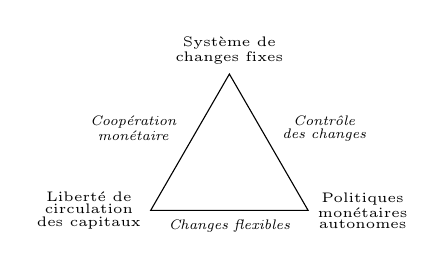
\begin{tikzpicture}
			\draw (0,0) node[left,align=center,execute at begin node=\setlength{\baselineskip}{0em}] {\tiny Liberté de\\ \tiny circulation\\ \tiny des capitaux} -- (2,0) node[right,align=center,execute at begin node=\setlength{\baselineskip}{0em}] {\tiny Politiques\\ \tiny monétaires\\ \tiny autonomes} -- (1,{sqrt(3)}) node[above,align=center,execute at begin node=\setlength{\baselineskip}{0em}] {\tiny Système de\\ \tiny changes fixes} -- cycle;
			\node[below] () at (1,0) {\tiny \em Changes flexibles};
			\node[left,align=center,execute at begin node=\setlength{\baselineskip}{0em}] () at (.45,{.6*sqrt(3)}) {\tiny \em Coopération\\ \tiny \em monétaire};
			\node[right,align=center,execute at begin node=\setlength{\baselineskip}{0em}] () at (1.55,{.6*sqrt(3)}) {\tiny \em Contrôle\\ \tiny \em des changes};
		\end{tikzpicture}
	\end{center}
	}
\longnewglossaryentry{theorie-des-marches-efficients}{name={Marchés efficients (théorie des\ldots)}}{%
	Développée par Eugene \textsc{Fama}, trois dimensions concourent à l'efficience des marchés\autocite[184]{Rae16} :
	\begin{enumerate}
		\item l'efficience opérationnelle : les produits financiers répondent aux besoins des agents, ce qui permet de réduire les coûts de transaction ;
		\item l'efficience informationelle : les prix des actifs concentrent toute l'information disponible sur les marchés ;
		\item l'efficience allocative : la comparaison entre le prix des actifs et leur rendement attendu permet d'orienter les capitaux vers les placements les plus rémunérateurs.
	\end{enumerate}
	}
\longnewglossaryentry{paradis-fiscal}{name={Paradis fiscal}}{
	L'OCDE retient quatre critères pour définir un paradis fiscal\autocite[196]{Rae16} :
	\begin{enumerate}
		\item une fiscalité faible ou nulle ;
		\item le secret bancaire et une absence de transparence ;
		\item l'absence d'échanges d'information avec les pays tiers ;
		\item l'absence d'activité économique réelle.
	\end{enumerate}

	L'OCDE a recensé une centaine de paradis fiscaux dans le monde, dont une dizaine en Europe.
	}
\newglossaryentry{ecoefficience}{name={Écoefficience},description={La baisse d'impact et de pollution par unité de marchandise produite\autocite[253]{Rae16}.}}
\newglossaryentry{empreinte-ecologique}{name={Empreinte écologique},description={La somme de la surface requise pour produire les ressources consommées par les sociétés humaines, de la surface occupée par les infrastructures et de la surface forestière nécessaire à la séquestration du CO\textsubscript{2} non absorbé par les océans\autocite[255]{Rae16}.}}
\newglossaryentry{pays-emergent}{name={Pays émergent},description={Pays en développement présentant un fort taux de croissance du PIB, un niveau relativement élevé d'industrialisation et d'exportation de produits industriels, un fort taux d'ouverture à l'extérieur et un marché intérieur en expansion\autocite[307]{Rae16}.}}
\longnewglossaryentry{defaillances-de-marche}{name={Marché (défaillances de\ldots)}}{%
	Au c\oe{}ur des théories de l'école du \textbf{bien-être} de Arthur Cecil \textsc{Pigou}, les défaillances de marché justifient l'action publique en ce qu'elle améliore la logique marchande et maximise le bien-être lorsque le marché ne permet pas de l'atteindre. On comptabilise à l'origine trois défaillances auxquelles est venue se rajouter une quatrième par les nouveaux keynésiens :
	\begin{enumerate}
		\item les externalités ;
		\item les biens collectifs ;
		\item les monopoles naturels ;
		\item les asymétries d'information (cf. George \textsc{Akerlof}).
	\end{enumerate}
	}
\longnewglossaryentry{risque-social}{name={Risque social}}{%
	Risque dont peuvent être victimes des individus, sans que leur responsabilité individuelle ne puisse \emph{a priori} être engagée. Les risques sociaux conduisent souvent à une interruption dans l'obtention du revenu tiré de la production, et il s'agit donc de subvenir aux besoins de la victime, puisqu'elle ne saurait être tenue responsable de son état.
	
	On dénombre cinq risques sociaux, et un sixième en discussion\autocite[362]{Rae16} :
	\begin{enumerate}
		\item la maladie ;
		\item les accidents du travail et maladies professionnelles ;
		\item la famille (\emph{e.g.} la grossesse) ;
		\item la vieillesse ;
		\item le chômage ;
		\item la dépendance.
	\end{enumerate}
	}
\longnewglossaryentry{lois-d-engel}{name={\textsc{Engel} (lois d'\ldots)}}{%
	Lois relatives à la structure de la consommation des ménages, établies par Ernst \textsc{Engel} (seule la première est véritablement attribuable à E. \textsc{Engel}) : le comportement moyen, en matière de consommation, se modifie avec le revenu. Cinq lois sont repérables :
	\begin{enumerate}
		\item lorsque le revenu augmente, les dépenses alimentaires augmentent également, mais moins vite que le revenu, ce qui signifie que leur part diminue dans le total des dépenses de consommation	\autocite{libres-a} ;
		\item la part des dépenses d'habillement et de logement reste stable avec le revenu, c'est-à-dire que ces dépenses augmentent au même rythme que le revenu ;
		\item la part des dépenses consacrées au logement, chauffage et éclairage est invariable quel que soit le revenu ;
		\item la part des dépenses diverses (santé, éducation, loisirs, s'accroît avec le revenu)\autocite[208]{BrE10b} ;
		\item l'accumulation du patrimoine est d'autant plus grande que le revenu est élevé\autocite[14]{Gau16f}.
	\end{enumerate}

	}
\newglossaryentry{optimum-de-pareto}{name={\textsc{Pareto} (optimum de\ldots)},description={Lorsque la distribution d'une ressource est telle que tout accroissement de la satisfaction d'un des consommateurs se traduirait par une diminution de la satisfaction d'au moins un des autres consommateurs.\autocite[22]{Gau16f}}}
\newglossaryentry{regle-du-maximin}{name={Maximin (règle du\ldots)},description={Chez John \textsc{Rawls}, elle consiste à \enquote{choisir la solution dont le plus mauvais résultat est supérieur aux plus mauvais résultats des autres\autocite[23]{Gau16f}}.}}
\longnewglossaryentry{etat-providence}{name={État-providence}}{%
	Dans une acception stricte, il s'agit de l'intervention de l'État dans le domaine social à travers le système de protection sociale, visant à instaurer une protection des individus par la collectivité contre les risques sociaux.
	
	Dans une acception plus large, il correspond à l'ensemble des interventions économiques et sociales de l'État\autocite[26]{Gau16f}.
	}
\newglossaryentry{ordre-politique}{name={Politique (ordre\ldots)},description={Désigne le champ d'activité dans lequel des membres d'une société, reconnus comme légitimes, peuvent contraindre la population à suivre des prescriptions. Il est un espace d'activité ayant trait au gouvernement\autocite[1]{Gau16l}.}}
\longnewglossaryentry{parti-politique}{name={Parti politique}}{%
	Pour Joseph \textsc{LaPalombara} et Myron \textsc{Weiner}, un parti politique est une organisation durable avec une articulation d'échelons locaux et national, animée d'une volonté de prendre et d'exercer le pouvoir (et non simplement d'influencer) et de rechercher, pour ce faire, le soutien populaire.
	
	Selon Max \textsc{Weber}, un parti doit être envisagé comme une sociation reposant sur un engagement formellement libre ayant pour but de procurer à leurs chefs le pouvoir et à leurs militants actifs des chances d'obtenir des avantages personnels et/ou de poursuivre des buts objectifs\autocite[8]{Gau16m}.
	}
\newglossaryentry{attitude-politique}{name={Attitude politique},description={Selon Pierre \textsc{Bréchon}, il s'agit d'une disposition générale, une \enquote{manière d'être en politique}. Elle est en principe plus pérenne et plus profonde que l'\textbf{opinion} et le \textbf{comportement politique}\autocite[1]{Gau16n}.}}
\longnewglossaryentry{competence-politique}{name={Compétence politique}}{%
	Une définition classique renvoie à trois éléments\autocite[4]{Gau16n} :
	\begin{enumerate}
		\item un intérêt revendiqué pour la politique ;
		\item une connaissance de l'univers politique comme univers spécialisé et institutionnalisé ;
		\item une capacité à penser selon des catégories politiques.
	\end{enumerate}

	Chez Pierre \textsc{Bourdieu}, la compétence politique correspond, dans une dimension objective à \enquote{la capacité plus ou moins grande de reconnaître la question comme politique et de la traiter en tant que tel en y répondant politiquement}\autocite[5]{Gau16n} et dans une domension subjective au \enquote{sentiment d'être plus ou moins légitime à intervenir en politique, à donner \enquote{son opinion}}\autocite[6]{Gau16n}.
	}
\longnewglossaryentry{indice-d-alford}{name={\textsc{Alford} (indice d'\ldots)}}{%
	Outil censé rendre compte de l'existence ou non d'un \emph{vote de classe}\autocite[12]{Gau16n}. Il repose sur un découpage très simplifié de la société entre ouvrier et non-ouvrier, et une distinction entre deux types de vote : à gauche / pas à gauche. Il se calcule en faisant la différence entre la part (en \%) des ouvriers votant à gauche et la part (en \%) des non-ouvriers votant à gauche. Si le résultat approche de 100, on a un vote de classe marqué.
	}
\longnewglossaryentry{indice-de-volatilite-electorale}{name={Volatilité électorale (indice de\ldots)}}{Il s'agit de mesurer les déplacements de voix d'une élection à l'autre. On calcule la valeur absolue de la différence entre les parts de voix obtenues par chaque parti d'une élection à l'autre. Puis ont fait la somme de ces différences. Enfin, on divise cette somme par 2 pour ne pas compter les déplacements de voix deux fois\autocite[12]{Gau16n}.}
\newglossaryentry{modele-de-la-seringue-hypodermique}{name={Seringue hypodermique (modèle de la\ldots)},description={Développé par Harold D. \textsc{Lasswell}, ce modèle considère que le message des médias est reçu, sans médiation et de manière indifférenciée, par le public\autocite[9]{Gau16o}. Kurt \textsc{Lewin} va complexifier le modèle en estimant que les messages émis peuvent être filtrés par des \emph{gatekeepers}, sorte de leaders dans les groupes sociaux qui exercent une sorte de contrôle sur les canaux de communication\autocite[10]{Gau16o}.}}
\newglossaryentry{loi-de-population}{name={Population (loi de\ldots)},description={Pour Thomas \textsc{Malthus}, l'accroissement des ressources ne permet pas de subvenir à l'accroissement des besoins de la population en raison du fait que la production de nourriture augmente de manière arithmétique (fonction linéaire du temps et rendements décroissants dans l'agriculture) alors que la population augmente à un rythme exponentiel\autocite[23]{DeG16b}.}}
\newglossaryentry{loi-des-debouches}{name={Débouchés (loi des\ldots)},description={Développée par Jean-Baptiste \textsc{Say}, \enquote{le seul fait de la formation d'un produit ouvre, dès l'instant même, un débouché à d'autres}, que l'on retient comme le fait que l'offre crée les conditions de sa propre demande\autocite[3]{DeG16c}.}}
\newglossaryentry{detour-de-production}{name={Détour de production},description={Une partie des revenus est détournée de la consommation pour être épargnée et financer ainsi l'investissement qui permettra à terme de produire encore plus de biens de consommation\autocite[18]{DeG16c}.}}
\newglossaryentry{anticipation-rationnelle}{name={Anticipation rationnelle},description={Théorisée par John \textsc{Muth}, une anticipation rationnelle qualifie le fait que les agents sont capables de tirer parti de toute l'information disponible pour former leurs anticipations, de sorte qu'en moyenne ils ne se trompent pas\autocite[23]{DeG16c}.}}
\longnewglossaryentry{politique-conjoncturelle}{name={Politique conjoncturelle}}{%
	Dans une optique keynésienne, on peut la définir comme l'ensemble des interventions de politique économique visant à réguler à court terme le niveau de la demande globale pour atteindre certains objectifs.
	
	Pour Nicholas \textsc{Kaldor}, les politiques conjoncturelles répondent à quatre objectifs finaux qui constituent un \enquote{carré magique}\autocite[2]{DeG16d} :
	\begin{enumerate}
		\item la \textbf{croissance économique}, mesurée par le taux de croissance du PIB ;
		\item l'\textbf{équilibre des échanges extérieurs}, mesuré par le solde courant rapporté au PIB ;
		\item le \textbf{plein emploi}, mesuré par le niveau du taux de chômage ;
		\item la \textbf{stabilité des prix}, mesurée par la variation de l'indice du niveau général des prix.
	\end{enumerate}
	}
\longnewglossaryentry{multiplicateur}{name={Multiplicateur}}{
	Le principe du multiplicateur keynésien tient dans le fait qu'une hausse ponctuelle de l'investissement (ou des dépenses publiques) va amener le PIB à augmenter de manière beaucoup plus forte. Il se formalise traditionnellement sous la forme ($k$ symbolise le multiplicateur) :
	\[\Delta Y = k \times \Delta I \]
	
	On repère ainsi plusieurs types de multiplicateurs\autocite[6]{DeG16d} :
	\begin{itemize}
		\item le multiplicateur de l'investissement avec $k = \frac{1}{1-c}$ ($c$ correspondant à la propension marginale à consommer) ;
		\item le multiplicateur des dépenses publiques avec $k = \frac{1}{1-c}$ (mais où la variation de l'investissement $\Delta I$ est substitué par la variation des dépenses publiques $\Delta G$) ;
		\item le multiplicateur en économie ouverte avec $k = \frac{1}{1-c+m}$ ($m$ correspondant à la propension marginale à importer) qui est plus faible que celui en économie fermée car une partie de la relance est consacrée à des biens et services importés ;
		\item le multiplicateur fiscal avec $k = \frac{-c}{1-c}$ (où la variation de l'investissement $\Delta I$ est substitué par la variation de l'imposition $\Delta T$) qui est moins important (et en sens inverse du multiplicateur des dépenses publiques) car les agents économiques peuvent choisir de ne pas modifier leur comportement ou au moins de ne pas consacrer à la consommation ou à l'investissement l'ensemble de la remise fiscale ;
		\item le multiplicateur d'un budget équilibré (selon le \textbf{théorème d'\textsc{Haavelmo}}) avec $\Delta Y = \frac{1}{1-c} \times \Delta G + \frac{-c}{1-c} \times \Delta T$.
	\end{itemize}
	}
\newglossaryentry{deficit-structurel}{name={Déficit structurel},description={Solde négatif des finances publiques qui ne tient pas compte de l'impact de la conjoncture (corrigé des cycles) sur la situation des finances publiques\autocite[15]{DeG16d}.}}
\newglossaryentry{production-potentielle}{name={Production potentielle},description={Niveau maximal de production soutenable à long terme sans tensions excessives dans l'économie, et plus précisément sans accélération de l'inflation\autocite[28]{DeG16d}.}}
\newglossaryentry{frontiere-technologique}{name={Frontière technologique},description={Niveau le plus avancé de la recherche technologique, elle peut se définir comme l'ensemble des technologies existantes les plus efficaces\autocite[28]{DeG16d}.}}
\newglossaryentry{effets-de-deplacements}{name={Effets de déplacement},description={Mis au jour par Alan T. \textsc{Peacock} et Jack \textsc{Wiseman}, ils correspondent au fait que les circonstances exceptionnelles des guerres lèvent la résistance à l'impôt, permettant en période de paix de financer de nouvelles activités publiques\autocite[2]{DeG16e}.}}
\longnewglossaryentry{impot}{name={Impôt}}{%
	Prélèvement obligatoire qui n'a pas pour contrepartie directe un service\autocite[13]{DeG16e}.
	
	Le calcul de l'impôt fait intervenir les concepts fondamentaux d'\textbf{assiette} (appelée aussi base fiscale elle correspond à la valeur de l'objet imposable à laquelle on applique le taux) et de \textbf{taux}. Le taux peut être \textbf{moyen} (correspondant au montant total de l'impôt dû divisé par la valeur de l'assiette) ou \textbf{marginal} (\emph{i.e.} le montant qui est prélevé sur le dernier euro de la base fiscale).
	
	Un impôt est dit \textbf{proportionnel} si son taux moyen ne varie pas quelle-que-soit l'étendue de la matière imposable ; à l'inverse il  est dit \textbf{progressif} (ou régressif) si son taux moyen augmente (ou diminue) avec la valeur de l'assiette\autocite[14]{DeG16e}.
	}
\newglossaryentry{vote-par-les-pieds}{name={Vote par les pieds},description={Analysé par Charles \textsc{Tiebout}, ce phénomène correspond au fait que les agents économiques révèlent leurs préférences individuelles en se déplaçant quand ils estiment que le poids des prélèvements obligatoires est trop important en regard des services rendus ce qui permet aux administrations de mieux cerner leurs attentes et mieux adapter leurs actions\autocite[16]{DeG16e}.}}
\newglossaryentry{regle-de-ramsey}{name={\textsc{Ramsey} (règle de\ldots)},description={Du nom de Franck P. \textsc{Ramsey}, elle consiste à moins taxer les bases fiscales les plus élastiques.}}
\longnewglossaryentry{triangle-de-harberger}{name={\textsc{Harberger} (triangle de\ldots)}}{%
	Il s'agit de la perte sèche de l'impôt. Les distorsions induites par la fiscalité réduisent le bien-être des agents car ils payent plus cher pour acheter le même bien, en raison de la fiscalité\autocite[18]{DeG16e}.
	
	\textsf{\textbf{Schéma\ldots}}
	}
\newglossaryentry{theoreme-de-stolper-samuelson}{name={\textsc{Stolper}--\textsc{Samuelson} (théorème de\ldots)},description={Le fait que les différents pays vont se spécialiser dans les produits utilisant en priorité les facteurs de production qu'ils possèdent en abondance, cette spécialisation va faire augmenter la rémunération des facteurs abondants\autocite[26]{DeG16e}.}}
\longnewglossaryentry{incidence}{name={Incidence}}{%
	Phénomène marquant les effets redistributifs des taxes et transferts. On peut repérer deux règles\autocite[31]{DeG16e} :
	\begin{enumerate}
		\item seuls les individus supportent le coût économique d'une taxe ou le bénéfice d'un transfert (l'impôt sur les sociétés n'est pas par exemple payé par les entreprises, et ne peut réellement peser que sur les actionnaires, les salariés ou les consommateurs) ;
		\item l'agent économique qui paie formellement une taxe ou qui reçoit un transfert n'est pas forcément celui qui paie réellement le prix économique de la taxe ou qui bénéficie du transfert.
	\end{enumerate}
	Il convient donc de distinguer l'incidence formelle de l'incidence économique.
	}
\newglossaryentry{equite-intergenerationnelle}{name={Équité intergénérationnelle},description={Elle renvoie à un traitement égal des générations au cours du temps et peut se définir comme une situation dans laquelle chaque génération bénéficie à chaque âge des mêmes ressources (ou niveaux de vie) que les autres générations aux mêmes âges\autocite[11]{DeG16f}.}}
\newglossaryentry{equite-intragenerationnelle}{name={Équité intragénérationnelle},description={Elle renvoie à un traitement égal des individus composant une génération donnée et se décline en une \textbf{équité horizontale} (traitement égal d'individus disposant du même niveau de revenus) et une \textbf{équité verticale} (redistribution entre individus disposant de niveaux de revenus différents)\autocite[11]{DeG16f}.}}
\newglossaryentry{regime-universel-par-points}{name={Régime universel par points},description={Dans le cadre des systèmes de retraite, il s'agit d'un régime à cotisations définies dans lequel les cotisations \emph{achètent} des points, unités de compte virtuelles, converties en pension à la liquidation, en fonction de la valeur du point\autocite[22]{DeG16f}.}}
\newglossaryentry{effet-rebond}{name={Effet rebond},description={Aussi appelé \enquote{paradoxe de \textsc{Jevons}}, il s'agit du fait que l'accroissement de l'efficacité technologique dans l'utilisation d'une ressource naturelle ne réduit pas la demande pour cette ressource, mais l'accroît au contraire. L'accroissement de l'efficacité énergétique engendre simultanément des économies d'énergie à court terme et une hausse de la consommation du bien à moyen terme qui peut annuler ces économies et finalement engendrer une plus grande consommation d'énergie\autocite[6]{DeG16h}.}}
\longnewglossaryentry{developpement-durable}{name={Développement durable}}{%
	Défini par le rapport \textsc{Brundtland} comme un \enquote{développement qui répond aux besoins du présent sans compromettre la capacité des générations futures de répondre aux leurs}. Il est la volonté de concilier le développement et la préservation de l'environnement en intégrant et reliant trois dimensions\autocite[19]{DeG16h} :
	\begin{enumerate}
		\item une dimension économique (la croissance des richesses doit être possible pour maintenir le niveau de bien-être des populations présentes) ;
		\item une dimension sociale (cette richesse doit être partagée dans le monde, entre les groupes sociaux) ;
		\item une dimension environnementale (les ressources de la planète doivent être préservées pour garantir que les générations futures puissent répondre à leurs besoins).
	\end{enumerate}
	}
\longnewglossaryentry{indicateur}{name={Indicateur}}{%
	On peut relever deux types d'indicateurs\autocite[28]{DeG16h} :
	\begin{enumerate}
		\item l'\textbf{indicateur agrégé} ou \textbf{synthétique} qui est construit à partir de l'agrégation des valeurs sur la base d'une unité de mesure commune (\emph{e.g.} le PIB ou l'empreinte écologique) ;
		\item l'\textbf{indicateur composite} qui résulte d'une moyenne pondérée d'indicateurs élémentaires éventuellement normalisés pour présenter de façon synthétique un phénomène multidimensionnel (\emph{e.g.} l'IDH).
	\end{enumerate}
	}
\newglossaryentry{instance-d-integration}{name={Intégration (instance d'\ldots)},description={Ensemble des structures, organisations et institutions qui in pour \enquote{fonction}, manifeste ou latente (cf. Robert K. \textsc{Merton}), de favoriser l'intégration\autocite[2]{Gau16e}.}}
\longnewglossaryentry{integration}{name={Intégration}}{%
	Serge \textsc{Paugam} propose une typologie de l'intégration par le travail qui va varier en fonction de la satisfaction et de la stabilité :
	\begin{center}
		\footnotesize 
		\begin{tabularx}{.4\textwidth}{X|X|X|X}
			\multicolumn{2}{c|}{} & \multicolumn{2}{c}{Satisfaction au travail}\\ \cmidrule{3-4}
			\multicolumn{2}{c|}{} & Oui & Non \\\midrule
			Stabilité dans l'emploi & Oui & Intégration assurée & Intégration laborieuse \\\cmidrule{2-4}
			et la famille & Non & Intégration incertaine & Intégration disqualifiante\\
		\end{tabularx}
	\end{center}
	}
\newglossaryentry{privatisation-de-la-famille}{name={Famille (privatisation de\ldots)},description={Chez Émile \textsc{Durkheim}, elle se traduit par le déclin des formes familiales caractérisées par la co-présence, dans le foyer, de plusieurs générations et le développement de la famille conjugale. La famille conjugale devient un \enquote{espace privé}, un \enquote{nous} primant sur les autres \enquote{nous} dont les interventions sont rejetées\autocite[3]{Gau16e}.}}
\newglossaryentry{inflation-scolaire}{name={Inflation scolaire},description={Pour Pierre \textsc{Bourdieu}, Jean-Claude \textsc{Passeron} ou encore Marie \textsc{Duru-Bellat}, en se généralisant, les diplômes perdent en partie de leur rendement social, alimentant encore la course au titre, dans une forme de cercle vicieux\autocite[9]{Gau16e}. Ce processus d'inflation scolaire est contesté par Tristan \textsc{Poullaouec}.}}
\newglossaryentry{multiculturalisme}{name={Multiculturalisme},description={Le fait que coexistent au sein d'une société des \emph{cultures} différentes et se pensant comme telles. Il s'agit d'un modèle d'organisation sociale qui reconnaît officiellement la diversité des cultures et des situations de certains groupes ou communautés, et leur attribue éventuellement des droits différents\autocite[26]{Gau16e}.}}
\newglossaryentry{minorite}{name={Minorité},description={Une minorité n'est pas un simple regroupement d'individus en ce qu'elle renvoie, au delà de sa singularité, à une disparité numérique dans laquelle un ensemble d'individus se trouve être en position d'infériorité par rapport à d'autres groupes au regard d'un ou plusieurs critères (ethnique, religieux, culturel, politique, linguistique, etc.) et entretenant des relations graduées, allant du conflit à la neutralité, avec les membres d'une population en situation majoritaire\autocite[27]{Gau16e}.}}